\chapter{Déductions et crédits d'emploi}
\section{Introduction et objectifs}
\subsection{Introduction}
Déductions et crédits qui s'appliquent au revenu d'emploi. On retrouve les déductions dans deux parties des T1 et TP-1: le calcul du revenu net et le calcul du  revenu imposable. De plus, nous étudierons certains crédits d'impôt non remboursables reliés à l'emploi qui peuvent être réclamés à l'étape~5 de la T1, ainsi qu'à la page 3 de la TP-1.


\subsection{Objectifs}
\begin{itemize}
	\item Expliquer ce qu'on entend par déduction pour travailleur et comment la réclamer;
	\item Réclamer la déduction pour un régime de pension agréé;
	\item Réclamer la déduction fédérale et le crédit d'impôt non remboursable du Québec relativement aux cotisations syndicales, professionnelles et autres cotisations semblables;
	\item Réclamer les dépenses d'emploi liées au travail à domicile en raison de la COVID-19;
	\item Expliquer comment le contribuable qui déménage pour occuper un emploi dans un nouveau lieu de travail peut réclamer des frais de déménagement;
	\item Réclamer la déduction pour remboursement de salaires ou de prestations d'assurance salaire;
	\item Réclamer la déduction pour le personnel des Forces canadiennes et des forces policières;
	\item Réclamer la déduction pour options d'achat de titres pour les employés;
	\item Réclamer la déduction pour ristourne reçue d'une coopérative;
	\item Réclamer la déduction pour revenu d'emploi gagné sur un navire;
	\item Calculer la cotisation que doit verser un employé au Régime de rentes du Québec (RRQ) et déterminer les cotisations versées en trop;
	\item Réclamer une déduction pour la cotisation bonifiée au RRQ sur un revenu d'emploi; 
	\item Calculer la cotisation que doit payer un employé au Régime québécois d'assurance parentale et déterminer les cotisations versées en trop;
	\item Calculer la cotisation que doit verser un employé à l'assurance-emploi et déterminer les cotisations versées en trop;
	\item Réclamer le montant canadien pour emploi;
	\item Réclamer le crédit d'impôt non remboursable pour pompiers volontaires ou volontaires participant à des activités de recherche et de sauvetage;
	\item Appliquer les règles régissant qui doit déclarer un revenu rétroactif de la Prestation universelle pour la garde d'enfants (PUGE) fédérale; 
	\item Réclamer le crédit d'impôt non remboursable pour les nouveaux diplômés travaillant dans une région ressource éloignée.
\end{itemize}


\subsection{Sujets du chapitre 3}
\begin{itemize}
	\item Déductions
	\item Déductions du revenu d'emploi
	\item Revenu net et imposable
	\item RRQ, RQAP et AE
	\item Crédits non remboursables pour revenu d'emploi
\end{itemize}



\section{Distinction entre déductions et crédits d'impôt}
\begin{intro}
	La première partie de ce chapitre concerne les déductions les plus communes qui sont reliées à l'emploi. L'application de ces déductions conduit au calcul du revenu net.
	
	La deuxième partie de ce chapitre concerne les déductions plus spécifiques qui sont aussi reliées à l'emploi. Celles-ci ne concernent que quelques contribuables. L'application de ces déductions fiscales spécifiques, conduit au calcul du revenu imposable.
	
	Enfin, la troisième partie de ce chapitre concerne les crédits d'impôt non remboursables qui sont reliés à l'emploi. Pour cette partie, nous verrons ceux pour le fédéral en particulier.
	
	Il est important de comprendre les différences entre les déductions et les deux types de crédits (remboursables et non remboursables) et comment ils sont utilisés dans le calcul de l'impôt sur le revenu.
\end{intro}
\begin{note}
	Les trousses d'impôt comprennent des guides qui fournissent des explications pour remplir chaque déclaration de revenus. Dans la transition vers le monde numérique, le guide fédéral a constaté une réduction des explications ligne par ligne. Si vous ne trouvez pas d'explication dans le guide, utilisez le champ de recherche sur le site Web de l'ARC et entrez le numéro de ligne.
	
	Cliquez sur le bouton ci-dessous pour afficher une liste complète de chaque ligne dans les étapes 3 à 6.
	
	\cat\href{https://www.canada.ca/fr/agence-revenu/services/impot/particuliers/sujets/tout-votre-declaration-revenus/declaration-revenus/remplir-declaration-revenus/deductions-credits-depenses/toutes-deductions-tous-credits-toutes-depenses.html}{Toutes les déductions, tous les crédits et toutes les dépenses}
\end{note}


\subsection{Déduction}
Une déduction réduit le revenu assujetti à l'impôt et, par conséquent, réduit en fin de compte l'impôt qu'une personne doit payer.

Il existe deux séries de déductions. Le premier ensemble réduit le revenu total dans le calcul du revenu net. Il se trouve à l'étape~3 - Revenu net de la T1 et à la section \og Revenu net \fg{} de la TP-1. 

Le deuxième ensemble de déductions réduit le revenu net dans le calcul du revenu imposable. Il se trouve à l'étape~4 - Revenu imposable de la T1 et à la partie \og Revenu imposable \fg{} de la TP-1.


\subsection{Crédits d'impôt non remboursables}
En ce qui concerne les crédits d'impôt non remboursables, ils servent à réduire l'impôt à payer plutôt que le revenu. 

Les crédits d'impôt ont la même valeur pour tous puisqu'ils sont accordés à un taux fixe pour tous les contribuables, peu importe leur revenu et leur taux marginal d'imposition. 

Les crédits d'impôt non remboursables sont déterminés pour la déclaration fédérale dans la partie des crédits d'impôt non remboursables à la section 5 de la T1, puis convertis au taux de 15~\%. D'autres crédits d'impôt non remboursables ont des taux différents, qui seront calculés plus tard, notamment dans la Partie C - Impôt fédéral net de l'étape~5 de la T1.

Au Québec, les crédits non remboursables peuvent être réclamés dans deux parties, les crédits d'impôt non remboursables et les revenus et cotisations à la page 3 du TP-1. Pour de nombreux crédits, le taux est de 14~\%, cependant il existe une fourchette de taux plus large que le fédéral variant entre 8~\% et
30~\% selon les crédits.

Si la valeur totale des crédits non remboursables est égale ou supérieure à l'impôt à payer, le contribuable ne tire aucun avantage du surplus. C'est pourquoi ils sont appelés non remboursables.

Au Québec, cependant, nous verrons dans un chapitre ultérieur comment un conjoint ayant un excédent de crédits non remboursables peut les transférer à sa conjointe si elle est en mesure d'utiliser l'excédent. 


\subsection{Crédits d'impôt remboursables}
Les crédits remboursables sont également utilisés pour réduire l'impôt à payer plutôt que le revenu. 

Toutefois, si un surplus est créé lorsque ces crédits sont appliqués à l'impôt à payer, ce surplus est retourné au contribuable sous forme de remboursement. 

Ceux-ci sont réclamés à l'étape~6 - \og Remboursement ou solde dû \fg{} de la T1 et \og Remboursement ou solde à payer \fg{} de la TP-1. 

Il existe deux types de crédits remboursables: 
\begin{itemize}
	\item Le premier type est des crédits pour des montants qu'un contribuable a déjà payés ou payés en trop. Le plus souvent, ces montants étaient déduits à la source; 
	\item Le deuxième type englobe les crédits d'impôt accordés par les gouvernements pour des programmes de redistribution des revenus ou de promotion de certains objectifs et politiques sociales.
\end{itemize}



\section{Calcul du revenu net}
\begin{intro}
	Le revenu net est déterminé en appliquant les déductions admissibles au montant du Revenu total. 
	
	Dans cette partie, vous découvrirez les déductions les plus courantes liées à l'emploi.
\end{intro}
Après avoir déterminé son revenu total, un contribuable doit identifier toutes les déductions auxquelles il est admissible.

Dans cette 1ère partie de chapitre, nous étudions les déductions qui sont reliées à un revenu d'emploi. Elles comprennent, entre autres:
\begin{itemize}
	\item La déduction pour travailleur, au Québec seulement;
	\item La déduction pour un régime de pension agréé;
	\item Les cotisations annuelles syndicales et professionnelles (sujet spécial);
	\item Déduction pour la cotisation bonifiée au RRQ sur un revenu d'emploi; 
	\item Les frais de déménagement.
\end{itemize}

Au fédéral, on déduit le remboursement des prestations de programmes sociaux à la ligne~23500.

Le revenu net est utilisé pour déterminer l'admissibilité du contribuable à certains crédits d'impôt et prestations sociales.

\begin{note}
	Sur les des déclarations fédérale et du Québec, le contribuable additionne toutes les déductions auxquelles il a droit, puis soustrait simplement le résultat du revenu total pour obtenir le revenu net.
	
	Étant donné que les déductions sur la déclaration fédérale et celle du Québec ne sont pas toujours les mêmes, il est tout à fait normal que les montants du revenu net soient différents.
\end{note}



\section{Déduction pour travailleurs}
\begin{intro}
	Le gouvernement du Québec offre à tous les contribuables ayant un revenu d'emploi une compensation financière afin d'assumer les petites dépenses quotidiennes reliées à l'emploi.
\end{intro}

Au Québec, sur la TP-1, le contribuable ayant un revenu d'emploi peut bénéficier d'une déduction pour travailleur correspondant à 6~\% du revenu de travail admissible, jusqu'à concurrence de \numprint{1315}~\$ pour l'année d'imposition 2023. 

Cette déduction se calcule sur la grille de calcul 201, présentée au tableau 3-1. Elle est réclamée à la ligne~201, réduisant ainsi le revenu net.

Les revenus de travail donnant droit à la déduction pour travailleurs comprennent:
\begin{itemize}
	\item Revenus d'emploi des lignes~101, 107 et si positif, ligne~105;
	\item Le montant net des subventions de recherche;
	\item Prestations du Programme de protection des salariés (sera discuté au chapitre 7);
	\item Montants reçus dans le cadre d'un projet d'incitation au travail.
\end{itemize}
\begin{note}
	Le revenu d'emploi composé uniquement d'avantages imposables obtenus en raison d'un emploi antérieur, ne constitue pas un revenu admissible aux fins de cette déduction. Le montant inscrit à la case~211 du relevé~1 doit être soustrait du montant inscrit à la ligne~101.
\end{note}
Sur la déclaration T1, l'équivalent de cette déduction est le Montant canadien pour emploi, qui est un crédit non remboursable.
\begin{note}
	Lorsque les revenus d'emploi sont supérieurs à \numprint{21916,67}~\$, la déduction maximum est de \numprint{1315}~\$.
\end{note}



\section{Régime de pension agréé (RPA)}
\begin{intro}
	Un \acrfull{rpa} est un régime de pension enregistré auprès de l'ARC conformément à la Loi de l'impôt sur le revenu. Le régime est mis en place par un employeur pour fournir un revenu de pension à ses employés au moment de leur retraite
\end{intro}
Les cotisations qui peuvent être versées à un RPA comprennent les cotisations pour services courants et celles pour services passés:
\begin{itemize}
	\item Service courant en 2023
	\item Service antérieur de 1990 à 2022
	\item Service antérieur pour 1989 et les années précédentes.
	\item 
\end{itemize}


\subsection{Déduction pour cotisations pour services courants}
Le montant retenu par l'employeur est indiqué aux cases~20 du feuillet T4 et D du relevé~1. Il peut également figurer sur un reçu émis par le syndicat du travailleur.

Une déduction peut être réclamée aux lignes~20700 de la déclaration T1 et 205 de la TP1.

Si un montant paraît à la case~52 du feuillet T4 et qu'aucun montant n'est inscrit aux cases~20 du T4 et D du relevé~1, cela signifie que l'employeur a versé toutes les cotisations au régime pour le bénéfice de l'employé.


\subsection{Cotisations pour services passés entre 1990 et 2022}
Au fédéral, les cotisations pour services passés rendus entre 1990 et 2021 sont généralement inscrites à la case~20 du T4. Lorsque la relation employeur-employé n'existe plus, les cotisations versées sont inscrites à la case~032 du feuillet T4A par l'administrateur du régime.

Au Québec,le montant de la cotisation pour services passés rendus après 1989 est indiqué à la case~D du relevé~1.

Les cotisations pour services passés rendus après 1989 sont entièrement déductibles seulement dans l'année où elles sont versées. Cela signifie que les cotisations pour services passés versées en 2022 doivent être déduites de la déclaration de revenus de 2022. Il n'existe aucun mécanisme permettant de demander la déduction pour les années suivantes.

Tout comme les cotisations pour services courants, elles sont réclamées aux lignes~20700 de la T1 et 205 de la TP1.

La déduction réclamée au Québec ne peut pas excéder celle demandée au fédéral.


\subsection{Cotisations pour services passés rendus avant 1989}
Les cotisations pour services passés rendus avant 1990 sont incluses à la case~20 du T4 et à la case~D du relevé~1. Elles sont également inscrites à la case~74 ou 75 du T4 et à la case complémentaire D-2 ou D-3 du relevé~1.

S'il n'y a aucune inscription aux cases~74 et 75 du T4 ou aux cases~D-2 et D-3 du relevé~1, alors le montant des cases~20 et D est entièrement déductible puisqu'il comprend uniquement des cotisations pour services courants ou pour services passés rendus après 1989.



\section{Exercice 3-1}
\setcounter{question}{0}
\begin{question}
	Quelle est la fonction des déductions?
\end{question}
Les déductions sont utilisées pour réduire le revenu.

Il existe deux séries de déductions. Le premier ensemble est utilisé pour réduire le revenu total afin de calculer le revenu net. Le second ensemble est utilisé pour réduire le revenu net afin de calculer le revenu imposable.

\begin{question}
	Quelle est la fonction des crédits d'impôt non remboursables?
\end{question}
Les crédits d'impôt non remboursables sont utilisés pour réduire l'impôt à payer.

\begin{question}
	Qu'est-ce qui différencie le traitement fiscal de la \og Déduction pour travailleur \fg{} de celui du \og Montant canadien pour emploi \fg{}? 
\end{question}
Au Québec, la déduction pour travailleurs est une déduction visant à réduire le revenu net du contribuable.

Le montant canadien pour emploi est un crédit d'impôt non remboursable permettant au contribuable de réduire son impôt à payer, lequel est établi à même son revenu imposable.

\begin{question}
	Durant l'année d'imposition 2023, en plus de sa cotisation pour son RPA de 460~\$ retenue sur son salaire, Barbara a également versé une cotisation de \numprint{6000}~\$ à son RPA pour des services passés rendus de 1994 à 1996.
\end{question}
\setcounter{sousQuestion}{0}
\begin{sousQuestion}
	Indiquez le montant qui sera inscrit aux cases~20 du T4 et D du relevé~1 émis par son employeur?
\end{sousQuestion}
\numprint{6460}~\$ (460~\$ + \numprint{6000}~\$)
\begin{sousQuestion}
	Est-ce que sa cotisation de \numprint{6000}~\$ pour services passés est entièrement déductible en 2023?  Quel montant peut-elle réclamer aux lignes~20700 de la T1 et 205 de la TP-1?
\end{sousQuestion}
Oui, ses cotisations pour services rendus après 1989 sont entièrement déductibles en 2024. Barbara peut réclamer \numprint{6400}~\$ (460~\$ + \numprint{6000}~\$) à la ligne~20700 de la T1 et à la ligne~205 de la TP-1.
\begin{sousQuestion}
	Au lieu de la déduire en 2023, Barbara peut-elle choisir de reporter sa cotisation de \numprint{6000}~\$ et réclamer la déduction dans une année subséquente?
\end{sousQuestion}
Non, si elle ne les réclame pas en 2023, elle ne pourra pas les réclamer dans une année subséquente.

Notez que les cotisations pour services passés antérieurs à 1990 sont assujetties à des règles différentes qui ne sont pas abordées dans ce cours.



\section{Régimes volontaires d'épargne-retraite (RVER) du Québec}
\begin{intro}
	Le but premier d'un régime volontaire d'épargne-retraite (RVER) est de donner accès à des régimes de retraite aux contribuables travailleurs autonomes et aux employés dont l'entreprise n'offre pas actuellement de régime de retraite enregistré.
\end{intro}
Les employeurs dont l'effectif dépasse un certain niveau sont tenus d'offrir la participation à un RVER s'ils n'offrent pas de régime de retraite enregistré ou de régime de retenues sur le salaire REER ou CELI.

Le contribuable établit sa propre cotisation au régime et l'employeur n'est pas tenu d'y participer. Toutefois l'employeur peut cotiser au RVER de son employé pourvu que celui-ci y participe également.

Contrairement aux régimes de retraite traditionnels, les RVER sont administrés par les institutions financières plutôt que par les employeurs, ce qui permet aux petites entreprises d'y participer sans exiger beaucoup de paperasse.

Le régime de pension agréé collectif (RPAC) est la contrepartie fédérale offerte aux provinces et territoires autres que le Québec.


\subsection{Traitement fiscal des cotisations à un RVER}
Les cotisations d'un employé à un RVER sont déductibles, mais pas sur la même ligne que le RPA. 

Toute contribution de l'employeur n'est pas imposable, mais elle diminue le montant que les contribuables peuvent cotiser à leur REER.

\qct\href{https://www.rrq.gouv.qc.ca/fr/retraite/rver/Pages/rver.aspx}{Le régime volontaire d'épargne-retraite (RVER)}

\cat\href{https://www.canada.ca/fr/agence-revenu/services/formulaires-publications/publications/t4040/reer-autres-regimes-enregistres-retraite.html}{REER et autres régimes enregistrés pour la retraite}, chapitre 8 - RPAC.



\section{Cotisations syndicales et professionnelles}
\begin{intro}
	Les contribuables qui paient des cotisations syndicales ou professionnelles peuvent bénéficier d'une déduction fédérale et d'un crédit d'impôt non remboursable au Québec pour les sommes qu'ils ont versées, pourvu que ces sommes se rapportent à leur emploi.
\end{intro}
\begin{note}
	Une caractéristique importante concernant la cotisation à un syndicat, à un ordre professionnel et à un comité paritaire:
	\begin{itemize}
		\item Une déduction est réclamée au fédéral;
		\item Un crédit d'impôt non remboursable est réclamé au Québec.
	\end{itemize}
\end{note}


\subsection{Cotisations admissibles}
Au fédéral et au Québec, les cotisations admissibles à la déduction et au crédit d'impôt comprennent notamment:
\begin{itemize}
	\item La cotisation annuelle versée à des associations professionnelles et syndicales. Les frais d'admission à un ordre professionnel ne sont pas déductibles, par exemple, les frais d'admission au Barreau, payés par un nouvel avocat;
	\item La cotisation versée à un office de professions, si le paiement est exigé par une loi provinciale ou territoriale;
	\item La cotisation obligatoire, incluant la prime d'une assurance responsabilité professionnelle, que le contribuable a versée pour lui permettre de conserver son statut professionnel reconnu par la loi; 
	\item La cotisation obligatoire effectuée à un comité paritaire ou consultatif (ou à un organisme semblable) ou à la Commission de la Construction du Québec (CCQ), comme l'exige la loi provinciale.
\end{itemize}

\subsubsection{Au Québec seulement}
Au Québec, les cotisations syndicales et professionnelles qui peuvent être réclamées comprennent également:
\begin{itemize}
	\item La cotisation à l'Association professionnelle des chauffeurs de taxi du Québec, pour permettre au contribuable de maintenir son permis de chauffeur de taxi;
	\item La cotisation annuelle à une association de salariés reconnue par le ministre du Revenu, ayant pour objets principaux l'étude, la sauvegarde et le développement des intérêts économiques de ses membres.
\end{itemize}

Si, pour un emploi donné, le contribuable réclame la cotisation à une association de salariés reconnue, il ne peut pas demander, pour cet emploi, le montant des cotisations effectuées à un syndicat, à un comité paritaire ou consultatif ou à un groupe semblable, à la Commission de la construction du Québec ou à l'Association professionnelle des chauffeurs de taxi du Québec.


\subsection{Traitement fiscal}
\subsubsection{case~44 du T4 et case~F du RL-1}
Les cotisations syndicales payées par retenue sur le salaire sont indiquées à la case~44 du T4 et à la case~F du relevé~1. 

Pour la déclaration fédérale, les montants de la case~44 ou du reçu peuvent être entièrement déduits à la ligne~21200 de la T1. 

Au Québec, les montants (case~F ou reçus) sont réclamés à titre de crédit d'impôt non remboursable à la ligne~397.1 du TP-1 au taux de 10~\% à la ligne~397.

\subsection{Assurance responsabilité professionnelle}
Au fédéral, ces primes peuvent être réclamées à la ligne~21200 de la T1. 

Cependant sur la TP-1, ces cotisations ne sont pas réclamées comme un crédit non remboursable, mais comme une dépense d'emploi à la ligne~207 de la TP-1, en utilisant le code 08 à la case~206.

\subsection{Remboursement de la TPS et de la TVQ}
Règle générale, la cotisation payée à une association professionnelle (excluant l'assurance responsabilité professionnelle) comprend la TPS et la TVQ. Si le contribuable veut réclamer le remboursement des taxes payées sur sa cotisation, il doit:

\begin{itemize}
	\item Au fédéral:
	\begin{itemize}
		\item Laisser le plein montant de la cotisation à la ligne~21200 de la T1;
		\item Remplir le formulaire suivant: GST 370 - Demande de remboursement de la TPS/TVH à l'intention des salariés et des associés;
		\item Demander le remboursement de la TPS à la ligne~45700 de la T1; 
		\item Le montant des deux taxes remboursées devient un montant imposable pour la prochaine année d'imposition. Le montant sera donc inscrit à la ligne~10400 de la T1.
	\end{itemize}
	\item Au Québec:
	\begin{itemize}
		\item Le montant inscrit à la ligne~397.1 doit exclure le montant payé pour la TPS et la TVQ;
		\item Remplir le formulaire suivant: VD-358 - Remboursement de la TVQ pour un salarié ou un membre d'une société de personnes; 
		\item Demander le remboursement de la TVQ à la ligne~459 de la TP-1.
		\item Le montant remboursé de la TVQ deviendra un montant imposable dans la prochaine année d'imposition, mais uniquement sur la déclaration fédérale. Le montant doit donc être inscrit à la ligne~10400 de la T1 de cette année.
	\end{itemize}
\end{itemize}

\cat\href{https://www.canada.ca/content/dam/cra-arc/formspubs/pbg/gst370/gst370-22f.pdf}{Demande de remboursement de la TPS/TVH à l'intention des salariés et des associés}

\qct\href{https://www.revenuquebec.ca/fr/services-en-ligne/formulaires-et-publications/details-courant/vd-358/}{Remboursement de la TVQ pour un salarié ou un membre d'une société de personnes}

Exemple: Cotisation professionnelle
\begin{itemize}
	\item T1
	\begin{description}
		\item[ligne~21200] Cotisation annuelle + TPS + TVQ + Assurance responsabilité + Contribution Office des professions du Québec
	\end{description}
	\item TP-1
	\begin{description}
		\item[ligne~397.1] Cotisation annuelle + Contribution Office des professions du Québec
		\item[ligne~397] 10~\% de la ligne~397.1
		\item[ligne~207]  Assurance responsabilité + code 08 à la case~206
	\end{description}
\end{itemize}



\section{Dépenses d'emploi}
\begin{intro}
	Les employés qui répondent à certains critères stricts peuvent déduire à la ligne~22900 les dépenses déterminées engagées pour gagner un revenu d'emploi. Un règlement général s'applique à tous les employés et aux employés des vendeurs à commission. Des règles spéciales s'appliquent aux employés de professions spécifiques telles que le transport, la foresterie, la musique, l'art, les métiers, les apprentis mécaniciens et le ministère religieux.
\end{intro}

En vertu du règlement général, les employés ne peuvent déduire les dépenses d'emploi admissibles que s'ils remplissent toutes les conditions suivantes:
\begin{itemize}
	\item Leur contrat de travail les oblige à payer les frais;
	\item Un avantage non imposable n'a pas été et ne sera pas reçu pour les dépenses; 
	\item Ils ont le formulaire T2200 - Déclaration des conditions de travail qui a été signé et certifié par l'employeur.
\end{itemize}

Les dépenses qui peuvent être déductibles comprennent le coût des fournitures, les frais de déplacement, les frais d'automobile et certaines dépenses liées à l'entretien d'un bureau ou d'un espace de travail à domicile.

Même si certains employés peuvent déduire les dépenses d'emploi, la grande majorité ne le sont pas. Seuls les particuliers qui remplissent les conditions particulières énoncées dans la Loi de l'impôt sur le revenu peuvent déduire les dépenses d'emploi. Pour tous les autres, la seule compensation disponible dans le cadre du régime d'impôt sur le revenu est le montant canadien pour emploi, un crédit non remboursable.


\subsection{Remboursement du revenu d'emploi}
À l'occasion, les contribuables peuvent être tenus de rembourser certains types de revenus d'emploi qu'ils ont inclus dans leur revenu dans une déclaration de l'année en cours ou de l'année précédente. Par exemple, un employé peut avoir à rembourser les prestations d'un régime d'assurance-salaire à la suite d'une décision subséquente de la Commission des accidents du travail. Dans de tels cas, le montant du remboursement peut être déduit à la ligne~22900 de la déclaration de revenus dans l'année du remboursement.

\arcg{21}



\section{Exercice 3-2}
\setcounter{question}{0}
\begin{question}
	Pierre Tremblay est rédacteur technique pour la compagnie Microsoft. Il a reçu un T4 et un relevé~1 indiquant qu'il a payé 105~\$ de cotisations syndicales. Il a également un reçu officiel indiquant qu'il a versé un montant de 70~\$ à la Société des auteurs au cours de l'année. Il n'y a eu aucune TPS ni TVQ sur les cotisations.
\end{question}

\setcounter{sousQuestion}{0}
\begin{sousQuestion}
	Est-ce que Pierre peut réclamer les sommes payées au titre des cotisations syndicales et professionnelles sur ses T1 et TP-1? Expliquez votre réponse.
\end{sousQuestion}
Oui, Pierre peut réclamer le montant payé à titre de cotisations syndicales et professionnelles, car elles sont liées à son revenu d'emploi.

\begin{sousQuestion}
	Quel montant peut-il déduire au titre des cotisations syndicales, professionnelles? 
\end{sousQuestion}
Pierre peut déduire 175~\$ (105~\$ + 70~\$) sur sa déclaration fédérale seulement. Dans la déclaration du Québec, il peut demander un crédit non remboursable (et non une déduction).

\begin{sousQuestion}
	Auxquelles lignes des T1 et TP-1 peut-il réclamer les cotisations payées?
\end{sousQuestion}



\section{Remboursement de salaires ou de prestations d'assurance salaire}
\begin{intro}
	Les contribuables sont parfois obligés de rembourser une partie de leur salaire ou de leurs indemnités de remplacement de salaire. Par conséquent, ils peuvent demander une déduction.
\end{intro}

À l'occasion, il arrive qu'un contribuable doive rembourser certains revenus d'emploi qui sont déclarés dans l'année courante ou dans une année antérieure. 

Par exemple, un employé peut devoir rembourser ses prestations d'assurance salaire lorsqu'il s'est vu accorder une indemnité pour accidents du travail par la Commission des normes, de l'équité, de santé et de la sécurité au travail (CNESST).

Dans de telles situations, le montant sera déclaré dans la case~77 du T4 et dans la case~A-3 ou à la case~O-4 du RL-1.

Des déductions peuvent être réclamées à la ligne~22900 de la T1 et à la ligne~207 de la TP-1 avec le code 10 dans la case~206.

La déduction sur la déclaration de revenus doit avoir lieu dans l'année où le contribuable a remboursé le montant, même si le montant reçu en trop a été encaissé dans les années antérieures.



\section{Revenu net}
Les déductions de vos déclarations fédérales et québécoises peuvent ne pas toujours concorder, ce qui entraîne des montants de revenu net différents.



\section{Calcul du revenu imposable}
\begin{intro}
	Déductions plus spécifiques qui sont aussi reliées à l'emploi. Celles-ci ne concernent que quelques contribuables dans des situations particulières.
\end{intro}

Le revenu imposable peut être réduit par d'autres déductions plus spécifiques:
\begin{itemize}
	\item Pour le personnel des Forces canadiennes et des forces policières;
	\item Pour les options d'achat de titres;
	\item Pour les ristournes reçues d'une coopérative; 
	\item Pour un revenu d'emploi gagné sur un navire.
\end{itemize}



\section{Déductions spécifiques}
\subsection{Personnel des Forces armées et policières}
La déduction est indiquée à la case~43 du T4 et peut être réclamée à la ligne~24400 de la T1.

La déduction est indiquée à la case~A-7 du relevé~1 et peut être réclamée à la ligne~297, code \og 23 \fg{} de la case~296 de la TP-1.

Le montant de la case~A-7 équivaut à la rémunération gagnée pendant le service à l'étranger, moins les cotisations à un RPA versé pendant cette période.


\subsection{Options d'achat de titres}
Un contribuable peut recevoir de son employeur une option d'achat de titres qui est une action du capital-actions de la société qui l'emploie. Le prix d'achat est déterminé d'avance. L'option devra être exercée dans un délai fixé.

Règle générale, l'employé a un certain temps pour exercer son option. Pendant ce temps, la valeur marchande des actions ou des unités peut fluctuer à la baisse ou à la hausse. Dans l'année où le contribuable exerce son option, si le prix de l'action ou de l'unité est moins élevé que sa valeur marchande au moment de l'exercice de l'option, la différence devient un avantage imposable pour l'employer. Heureusement, l'employé peut réclamer une \og Déduction pour options d'achat de titres \fg{}.

Dans la déclaration fédérale, l'avantage imposable est inclus à la case~14 du T4 du contribuable et inscrit dans la section \og Autres renseignements \fg{} où il est identifié par la case~38. Le montant de la déduction est inscrit à la case~39 ou 41 du même T4. Elle correspond à 50~\% de l'avantage imposable et est réclamée à la ligne~24900 de la T1.

Au Québec, l'avantage imposable est inscrit aux cases~A et L du relevé~1. La déduction (25~\% de l'avantage imposable) est inscrite aux cases~L-9 ou L-10 du relevé~1. La somme des entrées de toutes les cases~L-9 et L-10 est réclamée à la ligne~297, code \og 02 \fg{} à la case~296, du TP-1.

Si le contribuable reçoit des options sur titres d'un emploi à l'extérieur du Québec, c'est-à-dire qu'aucun relevé~1 n'est reçu, une déduction de 25~\% du montant de la case~38 du T4 peut encore être réclamée à la ligne~297, code \og 02 \fg{} à la case~296, du TP-1. Une copie du T4 doit être soumise avec la déclaration.


\subsection{Ristourne reçue d'une coopérative}
Les ristournes versées à un membre d'une coopérative admissible sous forme de parts privilégiées sont inscrites à la case~030 du T4A et à la case~O, code \og RL \fg{} à la case~\og Code (case~O) \fg{} du relevé~1. Le montant doit être déclaré à la ligne~13000 de la T1 et à la ligne~154, code \og 03 \fg{} à la case~153, de la TP-1.

Au Québec seulement, le contribuable peut réclamer une \og Déduction pour ristournes \fg{}. Le montant inscrit à la case~O-2 du relevé~1 peut être réclamé à la ligne~297, code \og 22 \fg{} de la case~296 du TP-1.


\subsection{Revenu d'emploi gagné sur un navire}
Au Québec seulement, un marin qui résidait au Québec en 2022 et qui possède une attestation du ministère des Transports du Québec peut bénéficier d'une déduction égale à 75~\% de la rémunération brute qu'un armateur admissible lui a versée dans l'année, pour une période où il a travaillé sur un navire affecté au transport international de marchandises. Il n'y a pas de déduction fédérale.

Si le propriétaire du navire a obtenu une attestation du Ministère des transports du Québec pour cet employé, le propriétaire doit inscrire le montant donnant droit à la déduction à la case~A-6 du relevé~1. Le contribuable peut demander la déduction à la ligne~297, code \og 08 \fg{} à la case~296, de la TP-1.


\subsection{Résumé des déductions spécifiques}
\begin{center}
	\begin{tabular}{|l|c|c|c|c|c|}
		\hline
		                  &  \textbf{T4}  &  \textbf{T1}   & \textbf{RL-1} & \multicolumn{2}{c|}{\textbf{TP-1}} \\ \cline{5-6}
		                  & \textbf{Case} & \textbf{Ligne} & \textbf{Case} & \textbf{Ligne} &   \textbf{Code}   \\ \hline
		Personnel des     &      43       &     24400      &      A-7      &      297       &        23         \\
		Forces armées     &               &                &               &                &     case~296      \\ \hline
		Options d'achat   &      39       &     24900      &      L-9      &      297       &        02         \\
		de titres         &      41       &                &     L-10      &                &     case~296      \\ \hline
		Ristourne reçue   &               &                &      O-2      &      297       &        22         \\
		d'une coopérative &               &                &               &                &     case~296      \\ \hline
		Marin             &               &                &      A-6      &      297       &        08         \\
		                  &               &                &               &                &     case~296      \\ \hline
	\end{tabular}
\end{center}

\rqg[s]{47-49}



\section{Revenu imposable}
Le revenu imposable du fédéral est différent de celui du Québec. Déductions qui peuvent être la cause de la différence:

\begin{itemize}
	\item La déduction de la cotisation syndicale ou professionnelle - au Fédéral seulement;
	\item La \og Déduction pour travailleur \fg{} - au Québec seulement;
	\item Options d'achat de titres (50~\% pour le fédéral et 25~\% pour le Québec); 
	\item Déduction pour revenu d'emploi gagné sur un navire - au Québec seulement.
\end{itemize}



\section{Exercice 3-3}
\setcounter{question}{0}
\begin{question}
	En janvier 2023, Mathieu Caron a obtenu une option d'achat de titres de la société qui l'emploie, ce qui lui a permis de faire l'acquisition de 250 actions au coût total de \numprint{2000}~\$. Au moment d'acheter les titres, leur juste valeur marchande était de 20~\$ par action. 
	
	Un avantage imposable de \numprint{3000}~\$ (250 x 12~\$) apparaît donc aux cases~38 et L de ses T4 et relevé~1 respectivement. 
	
	L'entreprise de son employeur n'est pas une PME poursuivant des activités innovantes. 
\end{question}
\setcounter{sousQuestion}{0}
\begin{sousQuestion}
	À quelles lignes de ses T1 et TP-1 Mathieu doit-il reporter l'avantage imposable?
\end{sousQuestion}
L'avantage imposable à la case~38 du T4 et à la case~L du relevé~1 est déjà inclus à la case~14 du T4 et à la case~A du relevé~1.

Les montants des cases~14 et A doivent être déclarés respectivement à la ligne~10100 de sa T1 et à la ligne~101 de sa déclaration TP-1.

\begin{sousQuestion}
	Quel est le pourcentage de l'avantage imposable que Mathieu peut réclamer comme déduction pour options d'achat de titres, au fédéral et au Québec?
\end{sousQuestion}
Au fédéral, Mathieu peut demander une déduction égale à 50~\% de l'avantage imposable qu'il a reçu.

Au Québec, il peut réclamer une déduction correspondant à 25~\% de l'avantage imposable qu'il a reçu.

\begin{sousQuestion}
	De quelle façon le montant de la déduction pour options d'achat de titres sera-t-il identifié sur ses feuillets de renseignements, au fédéral et au Québec?
\end{sousQuestion}
Au fédéral, le montant doit être inscrit à la case~39 ou 41 du T4. Au Québec, la déduction doit être inscrite soit à la case~L-9, soit à la case~L-10 du relevé~1, selon le type d'options. 

\begin{sousQuestion}
	À quelle ligne de ses déclarations T1 et TP-1 peut-il réclamer une déduction pour options d'achat de titres?
\end{sousQuestion}
Au fédéral, à la ligne~24900 de sa T1.

Au Québec, il peut demander une déduction à la ligne~297 de sa TP1, en utilisant le code 02 à la case~296.



\section{Impôt à payer sur le revenu imposable}
\begin{intro}
	Sur la déclaration T1 à l'étape~5, nous calculons l'impôt fédéral sur le revenu imposable suivi de la demande de tout crédit non remboursable applicable. Sur la déclaration TP-1, nous réclamons la plupart des crédits non remboursables avant de calculer l'impôt sur le revenu imposable. 
\end{intro}


\subsection{Grille de calcul de l'impôt}
La grille d'impôt du fédéral comporte cinq colonnes qu'on appelle \og Tranches d'imposition ».

\begin{note}
	Les taux d'imposition s'appliquent par tranche de revenu. De cette manière, un contribuable qui a un revenu très élevé n'aura pas à payer le taux le plus élevé sur tout son revenu. Il utilisera les taux applicables pour chaque tranche de revenu.
\end{note}



\section{Calcul des crédits d'impôt non remboursables}
\begin{intro}
	Crédits d'impôt non remboursables qui sont reliés à l'emploi.
\end{intro} 
\begin{itemize}
	\item Unique à la T1:
	\begin{itemize}
		\item Les cotisations de l'employé au Régime de rentes du Québec (RRQ);
		\item L'assurance-emploi (AE);
		\item Le Régime québécois d'assurance parentale (RQAP); 
		\item Le montant canadien pour emploi.
	\end{itemize}
	\item Unique à la TP-1:
	\begin{itemize}
		\item La cotisation syndicale, professionnelle ou autre;
		\item Crédit d'impôt pour la prolongation de carrière; 
		\item Le crédit d'impôt pour nouveau diplômé travaillant dans une région ressource éloignée.
	\end{itemize}
	\item Commun aux deux:
	\begin{itemize}
		\item Montant pour les pompiers volontaires et pour les volontaires en recherche et sauvetage.
	\end{itemize}
\end{itemize}

Sur la TP-1, Revenu Québec considère que le montant personnel de base tient compte des cotisations du contribuable au RRQ, à l'AE et au RQAP. Par conséquent, il n'y a pas de crédits distincts à réclamer.



\section{Régime de rentes du Québec (RRQ)}
\begin{intro}
	Ce sujet est d'une grande importance pour les contribuables du Québec. Avec des cotisations financières obligatoires dès l'âge de 18 ans par le biais de retenues sur les revenus d'emploi, le \acrfull{rrq} fait partie des actions préparatoires à la retraite.
\end{intro}

Le \acrfull{rpc} est la contrepartie fédérale offerte aux provinces et territoires autres que le Québec. 

Le Régime de rentes du Québec (RRQ) est obligatoire pour le contribuable dont le revenu annuel dépasse \numprint{3500}~\$.

Les cotisations aux régimes sont déterminées par la province d'emploi.
\begin{itemize}
	\item Si un contribuable réside et travaille au Québec, il doit cotiser au RRQ.
	\item Si un contribuable réside au Québec, mais travaille dans une autre province, il doit cotiser au RPC. Le formulaire fédéral RC381 est utilisé pour calculer la cotisation requise au lieu de l'annexe 8.
	\item Si un contribuable réside à l'extérieur du Québec, mais travaille au Québec, il doit cotiser au RRQ. Le même formulaire RC381 est utilisé pour calculer la cotisation requise au RRQ au lieu de l'annexe 8.
\end{itemize}


\subsection{Quand l'employeur doit-il retenir des cotisations au RRQ?}
\begin{note}
	Les gains admissibles, les gains assurables, le salaire admissible, le salaire assurable et la rémunération assurable ont tous la même signification. Ils représentent les revenus admissibles au calcul de la cotisation du RRQ.
	
	
	L'acronyme \acrshort{mga} veut dire \og Maximum de gains assurables ». Ce terme sera utilisé de temps à autre. C'est un lien direct avec le paragraphe précédent.
\end{note}

L'employeur doit retenir les cotisations du RRQ sur le salaire admissible qui donne droit à une pension pour le contribuable si celui-ci répond aux conditions suivantes:
\begin{itemize}
	\item Il est âgé de 18 ans et plus;
	\item Il occupe un emploi donnant droit à une pension;
	\item Il n'est pas considéré comme invalide selon le RRQ;
	\item Le contribuable doit toujours cotiser au RRQ s'il travaille, peu importe, son âge et même s'il reçoit des prestations de rente de retraite.
\end{itemize}

\subsection{Calcul de la cotisation au RRQ}
En 2023:
\begin{description}
	\item[Cotisation régulière] 5,40~\%
	\item[Cotisation supplémentaire] 1,00~\%
\end{description}

La cotisation de base que doit payer un contribuable au RRQ donne droit à un crédit d'impôt non remboursable qui peut être réclamé à la ligne~30800 de la T1. Il n'y a pas de crédit équivalent au Québec, car le montant personnel de base qui est réclamé à la ligne~350 de la TP-1 tient compte de la cotisation qui est versée au RRQ.

La cotisation supplémentaire donne droit à une déduction. Cette déduction peut être réclamée à la ligne~22215 de la T1 et à la ligne~248, avec le code \og 01 \fg{} à la case~248.1, de la TP-1.

\qct\href{https://www.rrq.gouv.qc.ca/fr/programmes/regime_rentes/Pages/regime_rentes.aspx}{Le Régime de rentes du Québec}


\subsection{Feuillets - T4 / RL-1}
\subsubsection{Salaire admissible au RRQ}
L'employeur doit inscrire le salaire admissible à la case~26 du T4 et à la case~G  du relevé~1. Le montant de la case~G du relevé~1 doit être reporté à la ligne~98.1 de la déclaration TP-1.

Si le montant de la case~26 du T4 est différent de celui de la case~G du relevé~1, le contribuable doit utiliser le montant de la case~G du relevé~1.

Si le salaire admissible a été exempté du RRQ pour toute l'année d'imposition, l'employeur doit inscrire un \og X \fg{} à la case~28 du T4 et inscrire \og 0,00~\$ \fg{} aux cases~26 du feuillet T4 et G du relevé~1.

\begin{note}
	Si l'employeur du Québec envoie un de ses employés travailler dans une autre province, ce dernier devra cotiser au RPC. L'employeur devra donc émettre un T4 avec le montant de la cotisation au RPC à la case~16. Il devra aussi émettre un relevé~1 avec le montant de la cotisation au RPC à la case~G-2 (case complémentaire).
\end{note}

\begin{note}
	Si le contribuable a deux emplois ou plus, les salaires admissibles donnant droit à une pension doivent être additionnés, mais la somme ne peut pas dépasser le maximum du salaire admissible établi par le RRQ.
\end{note}

\subsubsection{Cotisations au RRQ}
L'employeur, qui a retenu des cotisations au RRQ pour le contribuable, doit les inscrire à la case~17 du T4 et à la case~B du relevé~1. Le montant de la case~B du relevé~1 doit être reporté à la ligne~98 de la TP-1.

\subsubsection{Traitement fiscal des cotisations au RRQ}
Seule la cotisation de base est déclarée comme crédit non remboursable dans la T1, tandis que la cotisation supplémentaire est réclamée comme déduction sur les T1 et TP-1.

Le montant de la case~17 du T4 et la case~B du relevé~1 incluent la cotisation de base et la cotisation supplémentaire. Il est nécessaire de déterminer les montants séparément. L'annexe 8 est utilisée pour déterminer les deux cotisations ou la grille de calcul 248 est utilisée pour déterminer les deux cotisations.

Une fois que le fractionnement des cotisations a été déterminé, la cotisation de base doit être inscrite à la ligne~30800 à titre de crédit non remboursable et la cotisation supplémentaire (bonifiée) est inscrite à titre de déduction à la ligne~22215 de la déclaration T1 .

Sur la TP-1, seule la cotisation supplémentaire (bonifiée) est inscrite comme déduction à la ligne~248 avec le code \og 01 \fg{} à la case~248.1.


\subsection{Rémunération assujettie aux cotisations du RRQ}
En général, les rémunérations assujetties aux cotisations du RRQ comprennent:
\begin{itemize}
	\item Les salaires, traitements, primes, commissions ou autres rémunérations;
	\item La plupart des allocations et des avantages imposables en espèces ou autres qu'en espèces;
	\item Les honoraires liés à l'emploi ou à la charge; 
	\item Les pourboires et gratifications reçus pour services rendus.
\end{itemize}

Aux fins du RRQ, elles correspondent au total des montants qui figurent aux cases~A, Q, R et U du relevé~1. 

La case~R est utilisée si l'employeur a fait le choix irrévocable de participer au RRQ pour l'ensemble de ses employés indiens dont le travail est exclu du RRQ en raison de l'exemption d'impôt des Indiens pour le travail effectué sur une réserve. 

La case~U représente le salaire présumé avoir été versé en vertu d'une entente de retraite progressive.

Notez les points suivants:
\begin{itemize}
	\item Si le salaire admissible d'un contribuable est identique au montant de la case~A du relevé~1, le même montant sera inscrit dans la case~G. Ce montant devra également être inscrit à la case~26 du T4. Le montant de la case~G peut être différent de celui de la case~14 du T4. Cette situation peut se produire lorsqu'il y a un avantage imposable au Québec, mais non au fédéral, ou lorsqu'un avantage imposable indiqué sur le relevé~1 est supérieur à celui inscrit sur le T4;
	\item Si un employeur a versé des salaires différés à un dépositaire ou à un fiduciaire pour le compte de son employé, il doit en inscrire le total à la case~Q du relevé~1. Dans une telle situation, le montant inscrit à la case~G du relevé~1 correspond au total des cases~A et Q. Un montant égal à celui de la case~G est alors inscrit à la case~26 du T4;
	\item Lorsque l'employeur est présumé avoir versé un salaire en vertu d'une entente de retraite progressive pour laquelle un visa de Retraite Québec a été délivré, il doit en inscrire le montant à la case~U du relevé~1. De plus, il doit tenir compte de ce montant pour établir le montant des cotisations au RRQ. Par conséquent, le montant de la case~G peuvent correspondre au total des montants apparaissant aux cases~A et U du relevé~1. Un montant égal à celui de la case~G est alors inscrit à la case~26 du T4; 
	\item Si le salaire admissible est exonéré des cotisations au RRQ, le salaire et les avantages admissibles au RRQ peuvent être différents du montant de la case~A du relevé~1 ou de la case~14 du T4. Par conséquent, le montant inscrit à la case~G du relevé~1 et celui figurant à la case~26 du T4 devrait indiquer le salaire admissible réel.
\end{itemize}

\subsubsection{Gains exonérés}
Les gains suivants sont exonérés de cotisations au RRQ:
\begin{itemize}
	\item Le salaire versé à un employé pour un travail exclu du RRQ; 
	\item La valeur du logement fourni pendant l'année à un membre du clergé ou d'un ordre religieux, si une \og Déduction pour la résidence d'un membre du clergé \fg{} est réclamée;
	\item Le salaire versé à un employé avant et pendant le mois où il atteint 18 ans; 
	\item Le salaire versé à un employé au cours de la période où il reçoit une pension d'invalidité du RRQ.
\end{itemize}
\begin{note}
	Si tous les revenus de l'employé pour toute la période d'emploi au cours de l'année d'imposition sont exclus du RRQ, il n'y a aucune cotisation au RRQ versée. Dans ce cas, l'employeur n'inscrit aucun montant à la case~B du relevé~1, mais il doit indiquer 0,00~\$ à la case~G. Sur le T4, l'employeur n'inscrit aucun montant à la case~17, mais il doit inscrire 0,00~\$ à la case~26 du T4 et un \og X \fg{} à la case~28.
\end{note}

\subsubsection{Avantage imposable sur lequel aucune cotisation au RRQ n'a été retenue}
Le revenu d'emploi déclaré à la ligne~101 de la TP-1 peut inclure des avantages imposables sur lesquels aucune cotisation au RRQ n'a été retenue. Il peut s'agir notamment d'un \og Avantage imposable en nature », d'un \og Avantage relatif à un ancien emploi \fg{} ou d'une \og Compensation non incluse aux cases~A et L ».

Un \textbf{avantage imposable en nature} est un avantage consenti à un employé sans versement d'une somme d'argent ou chèque. Cet avantage représente un salaire admissible au RRQ pour l'employé et sa valeur doit être inscrite à la case~G-1 \og Avantage imposable en nature \fg{} du relevé~1. Le contribuable doit reporter le montant de la case~G-1 à la ligne~102 de la TP-1.

\textbf{L'avantage relatif à un ancien emploi}, tel que les primes versées par l'employeur à un régime privé d'assurance maladie au bénéfice d'un employé retraité, constitue un revenu d'emploi qui est inscrit à la case~A du relevé~1. Si le montant de la case~A est composé uniquement de la valeur d'un avantage que le particulier reçoit ou dont il a bénéficié dans l'année d'imposition en raison d'un ancien emploi, l'émetteur doit inscrire \og 211 \fg{} dans une case vierge du relevé~1, suivie du montant de la case~A. Aucune cotisation au RRQ n'a été retenue sur ce revenu.

Le montant de la case~211 du relevé~1 doit être inscrit à la ligne~102 du TP-1. Le contribuable peut choisir de verser des cotisations facultatives au RRQ. Le montant de la case~211 permet d'identifier les revenus qui ne donnent pas droit au contribuable à certaines déductions et crédits d'impôt.

\subsection{Calcul proportionnel}
Le salaire admissible au RRQ et l'exemption de base doivent être calculés au prorata si le contribuable est éligible au RRQ seulement pour une partie de l'année. 

Le calcul proportionnel obtenu a pour effet de diminuer le montant du salaire admissible qui doit être cotisé et, par conséquent, le montant de la cotisation requise.

Un calcul proportionnel doit être effectué si, en 2023, le contribuable:
\begin{itemize}
	\item A atteint 18 ans avant le mois de décembre. On utilise alors le nombre de mois dans l'année qui suivent le mois où il a atteint l'âge de 18 ans; 
	\item A commencé à recevoir des prestations d'invalidité du RRQ. On utilise alors le nombre de mois durant lesquels il n'a pas reçu de rente d'invalidité; 
	\item A cessé de recevoir des prestations d'invalidité du RRQ. On utilise alors le nombre de mois durant lesquels il n'a pas reçu de rente d'invalidité; 
	\item Est décédé avant le mois de décembre. On utilise le nombre de mois dans l'année jusqu'au mois du décès, y compris ce mois.
\end{itemize}

\begin{note}
	Le nombre de mois dans l'année où les prestations d'invalidité ont été reçues est indiqué à la case~21 du T4A(P) qui est le feuillet d'impôt sur lequel les sommes versées au contribuable sont déclarées.
\end{note}

\subsection{Cotisations payées en trop au RRQ}
Un contribuable peut se retrouver dans une situation dans laquelle il a versé trop de cotisations au RRQ. Cette situation peut survenir lorsqu'un contribuable possède plus d'un emploi.

\begin{note}
	\begin{enumerate}
		\item Si le trop-payé au RRQ n'est pas réclamé, un redressement ne peut être effectué que dans les quatre ans suivant l'année de la déclaration de revenus. Cette situation peut survenir lorsqu'un contribuable n'a pas produit sa déclaration.
		\item 	Il est possible d'avoir payé en trop au RRQ, même si le total des cotisations est inférieur au maximum.
	\end{enumerate}
\end{note}

\subsubsection{Si les sommes versées excèdent le maximum requis}
Si un contribuable n'a versé que des cotisations au RRQ et que le montant inscrit à la ligne~98 de la TP-1 dépasse la cotisation maximale de \numprint{4038,40}~\$, inscrivez le trop-payé à la ligne~452 de la TP-1.

\subsubsection{Trop-payé même si le montant maximum n'est pas dépassé}
Avec l'introduction de la cotisation additionnelle, le contribuable est tenu d'utiliser l'annexe 8 pour calculer la cotisation de base et la cotisation additionnelle.

En remplissant l'annexe 8, tout paiement en trop ou en moins sera identifié dans le résultat obtenu à la ligne~14 de l'annexe 8.

Si un contribuable a payé en trop le RRQ, le résultat du calcul à la ligne~14 de l'annexe 8 sera positif (voir Illustration 3-7) et devra être inscrit à la ligne~452 du
TP-1.

Le montant inscrit à la ligne~452 de la TP-1 est un crédit d'impôt remboursable. Le trop-payé, s'il excède la cotisation requise, est donc remboursable.

S'il y a eu un trop-payé en cotisations RRQ, il faudra modifier les montants qui sont inscrits aux lignes~22215 de la T1 et 248 de la TP-1. Il faudra aussi modifier le montant qui est inscrit à la ligne~30800 de la T1 au fédéral.

\begin{note}
	Il est important de s'assurer que les inscriptions suivantes ont été faites:
	\begin{itemize}
		\item À la ligne~98 de la TP-1: le total des cotisations au RRQ;
		\item À la ligne~98.1 de la TP-1: le total des salaires admissibles au RRQ.
	\end{itemize}
\end{note}


\subsection{Cotisations insuffisantes}
Le contribuable doit inscrire le montant des cotisations, tel qu'il est indiqué sur son ou ses relevés 1, à la ligne~98 de sa TP-1, et le total des gains admissibles à la ligne~98.1 de sa TP-1. 

Selon l'annexe 8, le montant que l'on doit inscrire à la ligne~30800 de la T1 est le montant de la ligne~7 de la Partie 2 de l'annexe 8, alors que le montant qu'on doit inscrire à la ligne~22215 de la T1 et à la ligne~248 de la TP-1 est celui de la ligne~10 de la Partie 2 de l'annexe 8.

Si, par inadvertance, le contribuable n'avait pas assez cotisé au RRQ, il n'est pas dans l'obligation de cotiser ce qui manque. Toutefois, s'il veut corriger l'erreur, il peut choisir de le faire en remplissant la Partie 4 de l'annexe 8.

\begin{note}
	Le montant cotisé au RRQ augmente vos prestations lorsque vient le temps de la retraite.
\end{note}



\section{Régime de l'assurance-emploi}
\subsection{Prestation spéciale d'AE}
Les travailleurs autonomes ne sont pas tenus de payer des cotisations à l'assurance-emploi, mais peuvent choisir de cotiser à un régime offrant des prestations spéciales.


\subsection{Cotisation maximale}
\begin{note}
	Le terme \acrfull{mga} est parfois utilisé pour décrire le revenu admissible dans le calcul des cotisations d'un contribuable.
\end{note}
Toutes les personnes employées, quel que soit leur âge, doivent payer des cotisations à l'assurance-emploi à partir de leur revenu d'emploi dès qu'elles commencent à gagner leur salaire, c'est-à-dire qu'il n'y a pas d'exemption de base ni de critère de limite d'âge. Par conséquent, aucun calcul au prorata.


\subsection{Retenues à la source}
L'employeur doit retenir les cotisations sur la paie de son employé. Il doit aussi inscrire les détails concernant les cotisations à la case~18 du T4 et à la case~C du relevé~1.

L'employeur doit remplir la case~24 du T4 (pas d'équivalent sur le relevé~1), en y inscrivant le montant total du salaire assurable de l'employé sur lequel il a retenu les cotisations à l'AE, jusqu'au maximum du MGA (\numprint{61500}~\$ en 2023). 

L'employeur doit inscrire \og 0,00~\$ \fg{} à la case~24 si l'employé n'a pas de salaire assurable et ajouter également un \og X \fg{} à la case~28 du T4.

Le montant de la case~24 du T4 n'est pas toujours le même que le montant de la case~14 du T4, car certains avantages imposables ne constituent pas des salaires assurables selon le programme d'assurance-emploi.


\subsection{Calcul de la cotisation}
Le montant de la cotisation requise correspond à la rémunération assurable multipliée par le taux établi de l'année d'imposition. Le taux établi par l'AE pour 2023 est de 1,27~\%.

\begin{note}
	Le taux de cotisation est plus bas au Québec que les autres provinces et territoires. 
	
	Les prestations d'assurance parentale hors Québec sont assumées par l'AE tandis qu'au Québec, elles sont assumées par le RQAP (sujet discuté plus loin dans ce chapitre).
\end{note}


\subsection{Traitement fiscal}
La cotisation versée à l'assurance-emploi doit être inscrite à la ligne~31200 de la T1.

Il n'y a pas de crédit équivalent au Québec, car le montant personnel de base qui est réclamé à la ligne~350 de la TP-1 tient compte de la cotisation qui est versée à l'AE.


\subsection{Trop-payé en cotisation d'assurance-emploi}
Si le total des primes payées excède la prime annuelle maximale, le contribuable peut réclamer l'excédent payé comme paiement en trop à la ligne~45000 de la T1.

Cette réclamation fournira un crédit d'impôt remboursable uniquement du gouvernement fédéral dans le cadre de l'administration du programme d'assurance-emploi.

Le trop-payé en cotisation à l'AE est calculé sur l'annexe 10 à la Partie C.

\begin{note}
	Si le trop-payé des cotisations AE n'est pas réclamé, un redressement peut être effectué jusque dans les trois dernières années excluant l'année de la déclaration de revenus. Cette situation peut survenir lorsque le contribuable n'a pas produit sa déclaration.
\end{note}


\subsection{Employé à faible revenu}
Un contribuable dont la rémunération assurable ne dépasse pas \numprint{2000}~\$ peut se faire rembourser les cotisations qu'il a payées. Il doit alors inscrire le montant des cotisations à la ligne~45000 de sa T1. Il n'y a aucune inscription à la ligne~31200 de sa T1 et aucune inscription à faire sur sa TP-1.



\section{Régime québécois d'assurance parentale}
\begin{intro}
	Ce programme offre des prestations aux employés qui prennent un congé de maternité, de paternité, d'adoption ou parental.
\end{intro}
Le \acrfull{rqap} remplace les prestations de maternité et les prestations parentales administrées antérieurement dans le cadre du programme fédéral d'assurance-emploi. 

Les prestations versées sont entièrement imposables. Le gouvernement fédéral utilise l'expression \acrfull{rpap} pour ce programme.

Au Québec, le RQAP assure aux travailleurs le versement d'une prestation imposable de maternité, de paternité, d'adoption ou d'un congé parental au cours duquel ils cessent d'être rémunérés.

Le RQAP est financé par les cotisations versées à Revenu Québec. Cette prime s'applique aux employeurs, aux employés et aux travailleurs autonomes. Du côté fédéral, le salarié peut réclamer un crédit d'impôt non remboursable pour les primes qu'il a payées. Au Québec, aucun crédit n'est accordé puisque le montant personnel de base est considéré comme incluant les différentes cotisations aux programmes sociaux (RRQ, AE et RQAP).


\subsection{Cotisations à payer}
Un contribuable (quel que soit son âge) doit payer des cotisations au Régime québécois d'assurance parentale (RQAP) sur ses revenus d'emploi, dès le premier dollar qu'il gagne. Aucun calcul au prorata n'est nécessaire.


\subsection{Retenues à la source}
L'employeur doit inscrire les détails concernant les cotisations à la case~55 du T4 et à la case~H du relevé~1. Le montant de la case~H du relevé~1 doit être reporté à la ligne~97 de la
TP-1.

L'employeur doit remplir la case~56 du T4 et la case~I du relevé~1, en y inscrivant le montant total du salaire assurable de l'employé sur lequel il a retenu les cotisations du RQAP. 

Il doit inscrire \og 0,00~\$ \fg{} s'il n'y a pas de rémunération assurable. Le montant de la case~56 n'est pas toujours le même que celui de la case~14 du T4, de même que la case~I n'est pas toujours la même que la case~A du relevé~1. Certains avantages imposables ne constituent pas une rémunération assurable aux fins du RQAP.

Il arrive à l'occasion que la case~56 du feuillet T4 soit laissée vide. Bien que l'employeur doit remplir cette case, vous pouvez utiliser le montant de la case~I du relevé~1 pour produire vos déclarations.


\subsection{Calcul de la cotisation}
Le montant de la cotisation requise correspond à la rémunération assurable multipliée par le taux établi de l'année d'imposition. Le taux établi par le RQAP pour 2023 demeure inchangé à 0,494~\%. 


\subsection{Traitement fiscal}
La cotisation versée au RQAP doit être inscrite à la ligne~31205 de la T1.

Il n'y a pas de crédit équivalent au Québec, car le montant personnel de base qui est réclamé à la ligne~350 de la TP-1 tient compte de la cotisation qui est versée au RQAP.

En tant que résidents du Québec, les contribuables doivent payer des cotisations au RQAP. Toutefois, le contribuable doit utiliser l'annexe 10 s'il travaille à l'extérieur du Québec ou à titre de travailleur autonome, pour la déclaration fédérale et la partie A ou B de l'annexe R pour le Québec pour déterminer sa cotisation au RQAP à payer.

\subsubsection{Trop-payé en cotisation RQAP}
Un trop-payé en cotisation au RQAP peut être demandé à la ligne~457 de la TP-1. 

Cette réclamation donnera un crédit d'impôt remboursable uniquement de Revenu Québec dans le cadre de l'administration du programme RQAP.

\begin{note}
	Si le trop-payé des cotisations au RQAP n'est pas réclamé, un redressement peut être effectué jusque dans les quatre dernières années excluant l'année de la déclaration de revenus. Cette situation peut survenir lorsque le contribuable n'a pas produit sa déclaration.
\end{note}


\subsection{Employés ayant un revenu de travail inférieur à \numprint{2000}~\$}

Le contribuable, dont les revenus admissibles au RQAP sont inférieurs à \numprint{2000}~\$, n'a aucune cotisation à payer au RQAP. Il peut réclamer le remboursement des cotisations qui ont été retenues sur son salaire, en inscrivant à la ligne~457 de sa TP-1, le montant qu'il a déjà inscrit à la ligne~97. Aucun montant ne doit être inscrit à la ligne~31205 de la T1.



\section{Contribuables du Québec travaillant dans une autre province ou un autre territoire}
\begin{note}
	Si un contribuable québécois travaille à l'extérieur du Québec, son employeur ne retiendra aucune cotisation au RQAP, mais il est tenu de payer une cotisation au RQAP.
\end{note}

Un contribuable qui réside et travaille au Québec doit verser des cotisations au RQAP. Ces cotisations sont déduites de sa rémunération. 

Si le même contribuable travaille à l'extérieur du Québec, aucune cotisation au RQAP ne sera retenue sur sa rémunération. Cependant, la cotisation retenue pour l'AE sera supérieure à la cotisation qu'ils paieraient au Québec. Cela s'explique par le fait que les cotisations provinciales d'assurance parentale sont incluses dans la cotisation d'assurance-emploi payable, de sorte que le taux de cotisation est plus élevé.

Puisque le contribuable réside au Québec, il doit payer sa part de cotisations au RQAP. 

Toutefois, en tant que résidents du Québec, le taux de cotisation applicable à leur rémunération assurable est inférieur et par conséquent, ils auront payé en trop au programme d'assurance-emploi.

Au lieu que le contribuable réclame un trop-payé à l'AE et paie séparément la cotisation requise au RQAP, il existe un mécanisme pour utiliser tout ou une partie du trop-payé à l'AE comme une partie ou la totalité de la cotisation au RQAP à payer.

L'annexe 10 (Parties B et C) et l'annexe R (Partie B) doivent être remplies.

Dans la pratique, l'ARC rembourse tout trop-payé à l'AE moins les cotisations que le contribuable est tenu de verser au RQAP. Ensuite, l'ARC transfère la cotisation du RQAP à Revenu Québec. Si le transfert de prime est insuffisant pour couvrir la prime requise au RQAP du contribuable, ce dernier devra payer le montant impayé à la ligne~439 de sa déclaration TP-1.



\section{Montant canadien pour emploi}
\begin{intro}
	Le montant canadien pour l'emploi est un crédit d'impôt non remboursable inscrit à la ligne~31260 à l'étape~5 de la partie B de la déclaration de revenus, qui peut réduire l'impôt fédéral d'un contribuable au taux de 15 %.
\end{intro}

Les employés peuvent demander le montant canadien pour emploi, selon le montant le moins élevé, à la ligne~31260:

\begin{itemize}
	\item \numprint{1368}~\$;
	\item Le total des revenus d'emploi déclarés aux lignes~10100 et 10400.
\end{itemize}

\begin{note}
	Le montant inscrit à la ligne~31260 correspond au montant du crédit d'impôt non remboursable.
	
	Le montant canadien pour emploi est calculé à 15~\%. Par conséquent, si un contribuable doit de l'impôt fédéral, le montant canadien pour emploi réduit l'impôt fédéral à payer jusqu'à un maximum de 205,20~\$.
\end{note}



\section{Volontaires dans les services d'urgence}
Afin d'encourager le recrutement, les pompiers volontaires et les volontaires en recherche et sauvetage ont droit à un crédit d'impôt non remboursable de \numprint{3000}~\$ au fédéral et de \numprint{5000}~\$ au Québec


\subsection{Admissibilité}
Pompier volontaire ou volontaire en recherche et sauvetage qui exécute au moins 200 heures.


\subsection{Services de pompier volontaire et de volontaire en recherche et sauvetage admissibles}
Un service de pompier volontaire et de volontaire en recherche et sauvetage admissible consiste principalement à:
\begin{itemize}
	\item Intervenir et être disponible en cas d'incendie ou en cas de situation d'urgence, de recherche et sauvetage;
	\item Assister à des réunions tenues par les services d'incendie ou par l'organisme de recherche et sauvetage;
	\item Suivre la formation requise liée à la prévention ou l'extinction des incendies ou aux services de recherche et sauvetage.
\end{itemize}


\subsection{Compensation financière non imposable}
Comme mentionné dans le chapitre 2, le pompier volontaire et le volontaire en recherche et sauvetage peuvent recevoir une compensation financière comme participant à des services d'urgence. La première tranche de 1 000 $ (1 315 $ au Québec) de cette compensation est exonérée d'impôt.

Au fédéral, elle est inscrite à la case~87 du feuillet T4. 

Au Québec, l'employeur a inscrit \og L-2 \fg{} dans une case vierge du relevé~1, suivi du montant.


\subsection{Traitement fiscal}
Le contribuable ne peut pas réclamer à la fois la partie exonérée d'impôt de la compensation et le crédit d'impôt pour les pompiers volontaires ou pour volontaire en recherche et sauvetage. 

S'il veut renoncer à l'exonération d'impôt et demander le crédit, le montant inscrit à la case~87 du T4 doit être ajouté au montant de la case~14. Au Québec, le montant relatif à la case~\og L-2 \fg{} du relevé~1 doit être ajouté au montant de la case~A.

Au fédéral, le Montant pour les pompiers volontaires (MPV) ou le Montant pour les volontaires en recherche et sauvetage (MVRS) peuvent être respectivement réclamés à ligne~31220 ou à la ligne~31240 de la T1. 

Au Québec, le crédit d'impôt est réclamé à la ligne~390 \og Crédit d'impôt pour pompiers volontaires ou pour volontaires en recherche et sauvetage \fg{} de la TP-1. De plus, un code doit être entré à la case~390.1 pour indiquer le type de service bénévole fourni. Si les deux services bénévoles ont été fournis, le contribuable peut entrer l'un ou l'autre code suivants:
\begin{itemize}
	\item 01 - Pompier volontaire; 
	\item 02 - Volontaire participant à des opérations de recherche et de sauvetage.
\end{itemize}

Au fédéral, le crédit d'impôt accordé est de 450~\$ (\numprint{3000}~\$ x 15~\%).

Au Québec, le crédit d'impôt accordé est de 700~\$ (\numprint{5000}~\$ x 14~\%).

\arcg{11}
\rqg[s]{21 et 56, 57}



\section{Exercice 3-4}
\setcounter{question}{0}
\begin{question}
	Qui doit cotiser au RRQ?
\end{question}
Tous les salariés résident du Québec de 18 ans et plus doivent cotiser au RRQ, ainsi que leurs employeurs. Il en va de même pour les travailleurs autonomes résidant au Québec.

\begin{question}
	Identifiez quatre types de gains exonérés du RRQ.
\end{question}
Les revenus suivants sont exonérés du RRQ:
\begin{itemize}
	\item Le salaire versé à un employé pour un travail exclu du RRQ;
	\item L'allocation reçu la résidence d'un membre du clergé ou d'un ordre religieux si la déduction pour résidence d'un membre du clergé a été ou peut être réclamée;
	\item Le salaire versé à un employé qui reçoit des prestations d'invalidité du RRQ; 
	\item Salaire versé à un employé durant le mois de son 18e anniversaire et les mois précédents.
	\item 
\end{itemize}

\begin{question}
	Quels sont les deux montants qui doivent être calculés proportionnellement lorsque la période de cotisation au RRQ d'un contribuable est plus courte que l'année entière?
\end{question}
Maximum des gains ouvrant droit à pension et exemption de base.

\begin{question}
	En vertu du RRQ, dans quelles circonstances doit-on effectuer un calcul proportionnel de ce montant? 
\end{question}
En vertu du RRQ, vous devez faire un prorata si le particulier:
\begin{itemize}
	\item A atteind 18 ans avant le mois de décembre de l'année d'imposition;
	\item A commencé à recevoir des prestations d'invalidité du RRQ au cours de l'année;
	\item A cessé de recevoir des prestations d'invalidité du RRQ au cours de l'année; 
	\item Si le contribuable bénéficiaire des prestations est décédé au cours de l'année.
\end{itemize}

\begin{question}
	Mariette, âgée de 38 ans, a reçu un relevé~1 indiquant \numprint{33000}~\S à la case~A et \numprint{1886,48}~\$ à la case~B. Un montant de \numprint{32650}~\$ figure à la case~G.
\end{question}
\setcounter{sousQuestion}{0}
\begin{sousQuestion}
	Quel est le montant de la cotisation requise au RRQ de Mariette? Démontrez vos calculs.
\end{sousQuestion}
Mariette doit cotiser \numprint{1865,60}~\$, calculé comme suit:
\[ (\numprint{32650} – \numprint{3 500}) \times 6,4~\% \]

\begin{sousQuestion}
	Son employeur a-t-il retenu la cotisation requise du sur la paie de Mariette? Sinon, expliquez ce que peut faire Mariette à ce sujet.
\end{sousQuestion}
Son employeur a retenu \numprint{1886,48}~\$, plus que le montant requis de \numprint{1865,60}~\$. Mariette peut réclamer le trop-payé de 20,88~\$ à la ligne~452 de sa TP-1.

\begin{sousQuestion}
	Effectuez les entrées appropriées aux lignes de la T1 et de la TP-1 de Mariette, indiquées ci-dessous.
	\begin{itemize}
		\item TP-1: ligne~98            
		\item TP-1: ligne~98.1         
		\item TP-1: ligne~248          
		\item TP-1: ligne~452          
		\item T1: ligne~30800        
		\item T1: ligne~22215
	\end{itemize}
\end{sousQuestion}
\begin{itemize}
	\item TP-1:
	\begin{description}
		\item[ligne~98] \numprint{1886,48}~\$
		\item[ligne~98.1] \numprint{32650,00}~\$
		\item[ligne~248] \numprint{291,50}~\$ \medspace \( ((\numprint{32650}~\$ - \numprint{3500}~\$) \times 1~\%) \)
		\item[ligne~452] \numprint{20,88}~\$
	\end{description}
	\item T1:
	\begin{description}
		\item[ligne~30800] \numprint{1574,10}~\$ \medspace \( (\numprint{29150}~\$ \times 5,4~\%) \)
		\item[ligne~22215] \numprint{291,50}~\$ \medspace \( (\numprint{29150}~\$ \times 1~\%) \)
	\end{description}	
\end{itemize}

\begin{question}
	Mark Phillips a reçu deux T4 affichant les renseignements suivants:
	
	\begin{center}
		\begin{tabular}{|c|c|c|}
			\hline
			   \textbf{case~14}    &   \textbf{case~18}   &    \textbf{case~24}    \\ \hline
			\numprint{32500,00}~\$ & \numprint{416,00}~\$ & \numprint{32500,00}~\$ \\ \hline
			\numprint{30100,00}~\$ & \numprint{388,80}~\$ & \numprint{30100,00}~\$ \\ \hline
		\end{tabular}
	\end{center}
\end{question}
\setcounter{sousQuestion}{0}
\begin{sousQuestion}
	Calculez la cotisation requise à l'AE et vérifiez s'il y a un trop-payé. Servez-vous de la Partie C de l'annexe 10.
\end{sousQuestion}
Cotisations combinées à l'AE \( = \numprint{416,00}~\$ + \numprint{388,80}~\$ = \numprint{804,80}~\$ \)

Prime maximale = 781,05~\$

Paiement en trop = 23,75~\$

\begin{sousQuestion}
	Effectuez les entrées appropriées aux lignes~31200 et 45000 de la déclaration T1 de de Mark.
\end{sousQuestion}
ligne~31200 de la T1: 781,05~\$

ligne~45000 de la T1: 23,75~\$

\begin{question}
	John Durham réside au Québec et a travaillé en Ontario. Il a reçu deux feuillets T4 de son employeur affichant les renseignements suivants:
	
	\begin{center}
		\begin{tabular}{|c|c|c|c|}
			\hline
			   \textbf{case~14}    &   \textbf{case~18}   &    \textbf{case~24}    & \textbf{case~55} \\ \hline
			\numprint{30350,00}~\$ & \numprint{475,58}~\$ & \numprint{30100,00}~\$ &     En blanc     \\ \hline
			\numprint{23000,00}~\$ & \numprint{363,40}~\$ & \numprint{23000,00}~\$ &     En blanc     \\ \hline
		\end{tabular}
	\end{center}
\end{question}
\setcounter{sousQuestion}{0}
\begin{sousQuestion}
	Est-ce que John peut réclamer son paiement en trop de l'assurance emploi à la ligne~45000 de son T1? Expliquez votre réponse.
\end{sousQuestion}
John a payé un total de 838,98~\$ en cotisations d'assurance-emploi. En tant que résident du Québec, la prime maximale à payer est de 674,37~\$. Par conséquent, le trop-payé perçu est de 164,61~\$.

Cependant, il doit aussi payer une prime au RQAP de 0,494~\% sur ses \numprint{53100}~\$ soit 262,31~\$.

Le trop-payé à l'AE deviendra simplement un paiement partiel sur sa cotisation au RQAP.

\begin{sousQuestion}
	Afin de calculer le trop-payé en cotisation à AE et de déterminer la cotisation RQAP, de quelles annexes doit-il se servir? Quelles parties doit-il compléter?
\end{sousQuestion}
Tout d'abord, Jean doit remplir la partie B de l'annexe 10 pour déterminer la cotisation requise au RQAP à la ligne~31210.

Deuxièmement, il doit remplir la partie C de l'annexe 10 pour établir la cotisation à l'AE requise pour le Québec et inscrire ce montant à la ligne~31200. Le paiement en trop sera inscrit à la ligne~45000.

Le montant de la ligne~31210 est ensuite soustrait du montant de la ligne~45000.

Si le résultat est positif, le trop-payé à l'AE est suffisamment important pour couvrir la cotisation requise au RQAP. Le montant requis est transféré à RQ et le solde sera remboursé à Jean à titre de trop-payé à l'AE.

Si le résultat est négatif, le trop-payé à l'AE est insuffisant pour couvrir la cotisation requise au RQAP. Tout le trop-payé à l'AE est alors transféré au RQ. Jean doit payer un montant supplémentaire sur sa TP-1 pour compléter son exigence de cotisation au RQAP.

Sur sa TP-1, Jean doit remplir la partie B de l'annexe R pour calculer le montant supplémentaire qu'il doit encore verser au RQAP. Ce montant doit être inscrit à la ligne~439 de la TP-1.

\begin{question}
	Charlotte Landry habite au 1275 rue Giguère, Québec, QC, G1P 1Z6 toute l’année. Son NAS est le 805 101 813 et sa date de naissance est le 5 février 1981. Elle est mariée à Gerald Landry, dont le NAS est le 805 101 821 et la date de naissance est le 15 juillet 1982, et son revenu total en 2023 était de \numprint{22480} \$. Charlotte et Gerald ne sont pas des travailleurs autonomes. Les Landrys n’ont pas d’enfants.

L’adresse courriel de Charlotte est clandry@videotron.ca et elle consent à recevoir de la correspondance en français par voie électronique uniquement.

Complétez les pages 1 des feuillets T1 et TP-1 de Charlotte Landry.
	
	\noindent
	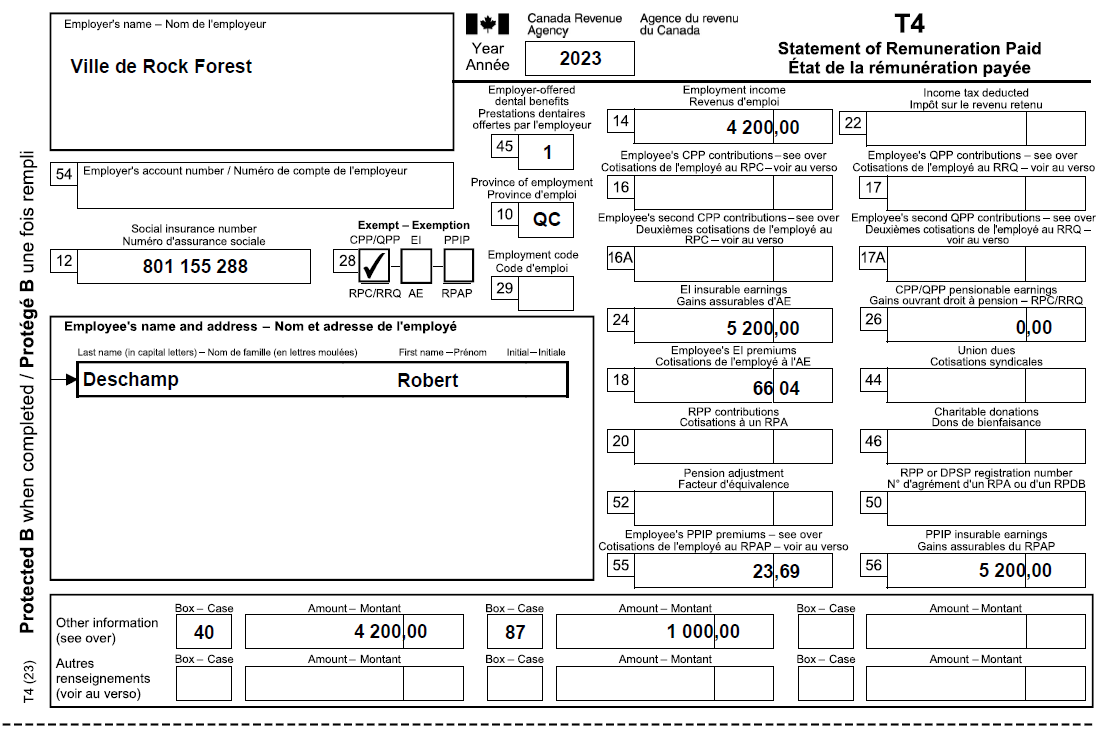
\includegraphics[width=\textwidth]{exercice/3-4/Q8/T4.png}
	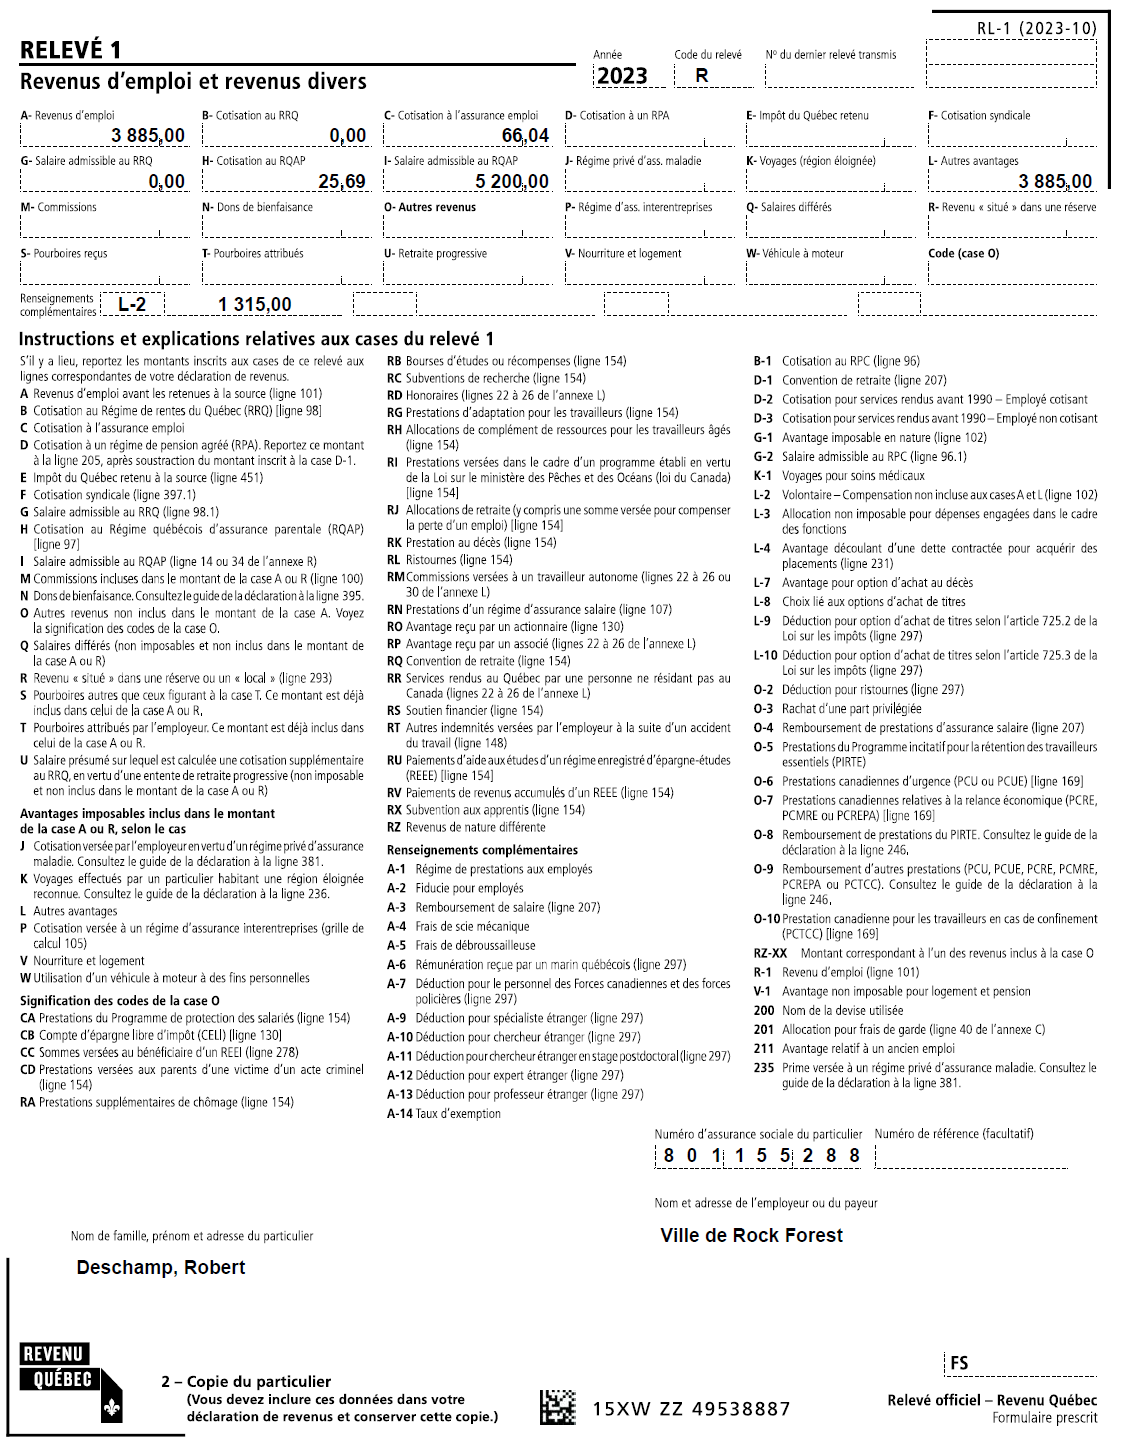
\includegraphics[width=\textwidth]{exercice/3-4/Q8/RL1.png}
\end{question}
Robert doit inscrire \numprint{5200}~\$ à la ligne 10100 de sa T1 et à la ligne 101 de sa TP-1. Un contribuable ne peut bénéficier à la fois de l'exonération d'impôt et du crédit d'impôt pour pompiers volontaires. S'il désire renoncer à l'exemption d'impôt au profit du crédit d'impôt, le montant inscrit à la case 87 du T4 doit être ajouté au montant de la case 14. Au Québec, le montant de la case L-2 du relevé 1 doit être ajouté au montant de la case A.



\section{Prestation universelle pour la garde d'enfants (PUGE)}
\begin{intro}
	Bien que ce programme ne soit plus offert depuis 2016, les dispositions du programme sont toujours valables pour les paiements rétroactifs.
\end{intro}
La \acrfull{puge} était un soutien financier direct, versée par le gouvernement fédéral.


\subsection{Traitement fiscal}
Le total des montants de la PUGE versés durant l'année est inscrit à la case~10 du feuillet RC62. 

Au fédéral, il doit être inscrit à la ligne~11700 de la déclaration T1 de l'époux ou conjoint de fait qui a le revenu net le moins élevé, peu importe celui qui a reçu les versements et le RC62. 

De plus, on doit en reporter le montant dans la partie \og Renseignements sur votre époux ou conjoint de fait », à la page 1 de la déclaration T1 de l'époux ou conjoint de fait ayant le revenu le plus élevé.

Au Québec, le total des versements reçus doit être inscrit à la ligne~278 de la déclaration TP-1 du conjoint au 31 décembre 2023 qui a le revenu net le moins élevé.

Au fédéral comme au Québec, si le revenu net du contribuable et celui de son époux ou conjoint de fait sont égaux, c'est celui qui a reçu les versements qui doit déclarer les montants reçus.

\subsubsection{Famille monoparentale}
Au fédéral, les chefs de famille monoparentale peuvent choisir d'inclure tous les montants de la PUGE qu'ils ont reçus dans le revenu de la personne à charge admissible pour laquelle ils ont demandé le montant.

S'ils font un tel choix, le montant de la case~10 du RC62 entre alors dans le revenu net de la personne pour laquelle ils demandent un montant pour une personne à charge admissible. 

Si cette personne produit une déclaration de revenus, elle doit déclarer le montant à la ligne~11700 de sa déclaration fédérale. Par ailleurs, les chefs de famille monoparentale doivent inscrire le même montant à la ligne~11701 de leur déclaration fédérale, au lieu de la ligne~11700.


\subsection{Remboursement de la prestation universelle pour la garde d'enfants}
Il est possible qu'un contribuable ou son époux ou conjoint de fait ait remboursé en 2023 un revenu de la PUGE qu'il a déclaré dans une année passée. Si c'est le cas, le montant figure à la case~12 du feuillet RC62. Cette personne peut réclamer une déduction correspondant au montant de la case~12 du feuillet RC62, à la ligne~21300 de la déclaration T1 de 2023.

Son époux ou conjoint de fait doit inscrire le montant du remboursement dans la partie \og Renseignements sur votre époux ou conjoint de fait », page 1 de la T1. 

Au Québec, la déduction peut être réclamée à la ligne~297, avec le code \og 24 \fg{} à la case~296, de la TP-1. Aucune autre inscription ne doit être faite sur cette déclaration.



\section{Crédit d'impôt pour nouveau diplômé travaillant dans une région ressource éloignée du Québec}
Le crédit est calculé sur le formulaire TP-776.1.ND Crédit d'impôt pour nouveau diplômé travaillant dans une région ressource éloignée et est réclamé à la ligne~392 de la TP-1.

\qct\href{https://www.revenuquebec.ca/fr/services-en-ligne/formulaires-et-publications/details-courant/tp-776-1-nd/}{Crédit d'impôt pour nouveau diplômé travaillant dans une région ressource éloignée }

Le montant cumulatif de ce crédit d'impôt non remboursable est de \numprint{10000}~\$ pour les nouveaux diplômés titulaires d'un diplôme de niveau postsecondaire (collégial ou universitaire) qui ont commencé à occuper un emploi dans les 24 mois suivants la date à laquelle ils ont complété leur formation ou obtenu leur diplôme.

\begin{note}
	les diplômes d'études professionnels, les attestations de formation professionnelle et les attestations de spécialisation professionnelle décernés par le Ministère de l'Éducation, du Loisir et du Sport ne font pas partie des diplômes reconnus. L'obtention d'un tel diplôme permet encore l'admissibilité au crédit d'impôt cumulatif de \numprint{8000}~\$.
\end{note}



\section{Crédits d'impôt non remboursables}
La partie des crédits d'impôt relatifs à l'emploi n'est qu'une introduction aux nombreux crédits d'impôt à venir.



\section{Frais de déménagement}
Le contribuable qui déménage pour occuper un emploi dans un nouveau lieu peut réclamer des frais de déménagement aux lignes~21900 de la T1 et 228 de la TP-1.


\subsection{Comment faire la réclamation}
Le contribuable doit utiliser les formulaires T1-M au fédéral et TP-348 au Québec.

Il n'est pas nécessaire d'avoir trouvé un emploi au moment du déménagement. Toutefois, la réclamation du contribuable peut être refusée lorsque le but principal du déménagement n'était pas de se trouver un emploi ou qu'il a pris beaucoup de temps avant de s'en trouver un.

Si les deux conjoints déménagent pour occuper de nouveaux emplois ou créer de nouvelles entreprises, les frais de déménagement peuvent être partagés entre eux.

Si un employeur mute un employé à un nouvel endroit et paie une partie ou la totalité des frais de déménagement, ces mêmes frais ne peuvent être déduits par l'employé. Seuls les frais de déménagement admissibles en sus de ceux payés ou payables par l'employeur ou pour lesquels le contribuable n'est pas remboursé sont déductibles.

Un contribuable n'est pas considéré comme ayant changé son lieu de résidence s'il déménage pour une période temporaire et continue de conserver sa résidence pour que sa famille y demeure pendant qu'il est parti.


\subsection{Condition relative à la distance}
La nouvelle résidence doit permettre au particulier de se rapprocher d'au moins 40 kilomètres du nouveau lieu de travail, comparativement à la distance entre l'ancienne résidence et le nouveau lieu de travail.


\subsection{Frais admissibles}
\begin{itemize}[label=\twemoji{check mark button}]
	\item Les frais de transport des effets personnels, y compris l'emballage, le déplacement, l'entreposage et les assurances;
	\item Les frais de déplacement vers la nouvelle résidence pour le contribuable et sa famille, y compris les frais de voyage, de repas et de logement pendant le trajet;
	\item Les frais de subsistance (repas et logement) pour le contribuable et les membres de sa famille pour séjourner à proximité de l'ancienne et/ou de la nouvelle résidence (période maximale de 15 jours);
	\item Les frais de résiliation du bail à l'ancienne résidence, à l'exclusion de tout loyer payé pendant qu'il y demeurait;
	\item Les frais accessoires consécutifs au déménagement, y compris le coût de la révision des documents juridiques pour tenir compte du changement d'adresse, le coût du remplacement des permis de conduire et des certificats d'immatriculation des véhicules non commerciaux (sauf les assurances) et les frais de branchement et de débranchement exigés par les services publics;
	\item Les frais d'entretien de l'ancienne résidence si elle est demeurée vacante et que des efforts ont été faits en vue de la vendre, y compris les intérêts hypothécaires, impôts fonciers, primes d'assurance, chauffage, électricité et les services publics, jusqu'à l'occurrence de \numprint{5000}~\$;
	\item Les frais relatifs à la vente de l'ancienne résidence, y compris la pénalité pour l'acquittement d'une hypothèque avant l'échéance, la commission versée à l'agent immobilier, les honoraires payés au notaire ou à l'avocat, les frais de publicité, les frais d'arpentage, etc.; 
	\item Les frais relatifs à l'acquisition de la nouvelle résidence, seulement si l'ancienne résidence a été vendue suite au déménagement (frais juridiques, droits de mutation (taxe municipale de bienvenue), enregistrement du droit de propriété au Bureau de la publicité des droits). Si c'est une première maison, ces frais ne sont pas admissibles.
\end{itemize}


\subsection{Frais de déménagement non déductibles}
\begin{itemize}[label=\twemoji{cross mark}]
	\item Les frais de transport engagés avant le déménagement pour la recherche d'un emploi, d'une résidence au nouvel endroit ou pour tout autre motif;
	\item Le coût des travaux effectués pour faciliter la vente de l'ancienne résidence et les pertes subies lors de la vente;
	\item La valeur des articles que les déménageurs refusent de prendre (plantes, aliments surgelés, munitions, peinture, carburant, huile, produits de nettoyage);
	\item Les frais qui ont été payés pour nettoyer ou réparer une résidence louée afin de respecter les exigences du propriétaire ou pour remplacer des biens à usage personnel (remise, bois de chauffage, rideaux, moquettes);
	\item Le coût de l'acheminement du courrier à la nouvelle adresse;
	\item Le coût des transformateurs et adaptateurs pour les appareils électroménagers;
	\item Les frais d'inspection de véhicules et le test d'émission; 
	\item Les frais de vente de l'ancienne résidence, si le contribuable en a retardé la mise en vente pour des raisons d'investissement ou de meilleures conditions de vente.
\end{itemize}


\subsection{Calcul des frais de déplacement et des frais de repas lors de l'hébergement temporaire}
Le contribuable a le choix entre deux méthodes (simplifiée ou détaillée) pour calculer les dépenses pouvant être réclamées pour les frais de repas et les frais de déplacement de l'ancienne résidence à la nouvelle résidence. Revenu Québec utilise les mêmes taux pour la méthode simplifiée que l'ARC.

\subsubsection{Calcul des frais de repas}

\paragraph{Méthode simplifiée}
Le contribuable qui choisit la méthode simplifiée peut réclamer un montant fixe de 23~\$ par repas, par personne, jusqu'à un maximum de 69~\$ par jour sans avoir à produire de reçus. 

La méthode simplifiée peut être utilisée pour les repas consommés pendant le trajet vers le nouveau lieu de résidence et pendant la période maximale de 15 jours pour le séjour dans un logement temporaire. 

Le contribuable doit être en mesure de fournir des pièces justificatives pour établir la durée de location du logement.

\paragraph{Méthode détaillée}
Selon cette méthode, un contribuable peut réclamer les frais de repas qu'il a payés, en fonction de ses reçus (à coût raisonnable), qu'il doit conserver.

\subsubsection{Calcul des frais de kilométrage}
Le contribuable qui utilise sa voiture personnelle peut choisir la méthode simplifiée ou la méthode détaillée pour calculer les frais de véhicule.

\begin{note}
	Le contribuable n'a aucune obligation de choisir la même méthode pour le calcul des frais de repas et de kilométrage. Il est tout à fait possible de choisir une méthode pour réclamer les frais de repas et l'autre méthode pour les frais de kilométrage.
\end{note}

\paragraph{Méthode simplifiée}
Le contribuable peut réclamer les dépenses relatives à son véhicule en utilisant un taux par kilomètre parcouru. Pour le Québec, le taux de 2023 est de 0,575~\$ par kilomètre parcouru.

Le taux en question varie selon la province ou le territoire d'où provient le déménagement. Par conséquent, les déménagements à l'intérieur du Québec seraient à un taux de 0,575~\$ par kilomètre, tandis qu'un déménagement en provenance de l'Ontario serait à un taux de 0,59~\$ par kilomètre.

Bien que le contribuable qui utilise la méthode simplifiée ne soit pas obligé de conserver des reçus, il doit toutefois conserver un registre du kilométrage parcouru relativement au déménagement.

\paragraph{Méthode détaillée}
Le contribuable peut utiliser cette méthode pour réclamer les frais de fonctionnement et les frais de propriété d'une automobile utilisée à des fins de déménagement (pourcentage d'utilisation du véhicule à des fins du déménagement). Il doit tenir un registre du kilométrage parcouru et conserver tous ses reçus.

Les frais de fonctionnement incluent l'essence, l'huile, les pneus, l'immatriculation, les primes d'assurance, l'entretien et les réparations du véhicule. Les frais de propriété du véhicule comprennent les taxes, les intérêts sur emprunt pour financer son achat et l'amortissement. 

\subsection{Limite du revenu admissible net}
Les frais de déménagement peuvent être déduits seulement du revenu net gagné au nouveau lieu de travail. 

Pour déterminer le revenu net admissible au nouveau travail, le contribuable doit d'abord calculer le total des revenus gagnés au nouveau lieu de travail comme suit:
\begin{itemize}
	\item Le montant inscrit sur le feuillet T4 relié au nouveau lieu de travail et déclaré à la ligne~10100. La même condition s'applique pour le relevé~1 et le montant est déclaré à la ligne~101 de la TP-1; plus
	\item Le revenu d'emploi gagné sur le feuillet T4A et déclaré à la ligne~10400. La même condition s'applique pour le relevé~1 et le montant est déclaré à la ligne~107 de la TP-1; plus
	\item Le revenu net d'entreprise si travailleur autonome; plus
	\item Les prestations du Programme de protection des salariés.
\end{itemize}

Par la suite, le contribuable doit réduire le total de ces montants en utilisant les déductions admissibles suivantes qu'il réclame:
\begin{itemize}
	\item Au Québec seulement, la déduction pour travailleur (ligne~201);
	\item La cotisation versée à un RPA reliée au nouvel emploi aux cases~20 du T4 et D du relevé~1 (lignes~20700 de la T1 et 205 de la TP-1);
	\item Au fédéral, la cotisation syndicale, professionnelle ou semblable reliée au nouvel emploi (ligne~21200 de la T1);
	\item Tous les autres frais admissibles reliés au nouveau lieu de travail, habituellement inscrits aux lignes~22215, 22900, 23100 et 23200 de la T1 et aux lignes~207, 236, 248 et 250 de la TP-1.
\end{itemize}

\begin{note}
	Les déductions pour les travailleurs (ligne~201) et les cotisations bonifiées au RPC/RRQ (lignes~22215 et ligne~248) sont calculées en fonction du revenu gagné total, provenant à la fois de l'emploi à l'ancien et au nouvel emplacement. 
	
	Par conséquent, un prorata de ces montants doit être calculé. 
	
	Utilisez la valeur du revenu gagné au nouvel emplacement / le revenu gagné total.
\end{note}

Par ailleurs, le calcul du revenu net au nouveau lieu de travail n'est pas nécessaire si le revenu brut à cet endroit est substantiellement plus élevé que les frais de déménagement. Dans une telle situation, il suffit d'entrer le  montant des revenus d'emplois des lignes~10100 et 10400 de la T1 et ceux des lignes~101 et 107 de la TP-1, plus les prestations du Programme de protection des salariés aux lignes~10400 de la T1 et 154 de la TP-1, sur les déclarations appropriées.


\subsection{Réclamation des frais de déménagement}
Au fédéral, le contribuable doit utiliser le formulaire T1-M afin de calculer et réclamer la déduction pour frais de déménagement à la ligne~21900 de la T1. Il doit le conserver, ainsi que les reçus et les autres pièces justificatives, afin de pouvoir les fournir à l'ARC sur demande.

Au Québec, le contribuable doit compléter le formulaire TP-348 et réclamer la déduction à la ligne~228 de la TP-1. Il doit joindre le formulaire à sa déclaration provinciale. Il doit conserver les reçus relatifs aux frais qu'il réclame pour pouvoir les fournir sur demande.


\subsection{Report des frais de déménagement inutilisés d'une année précédente}
Il arrive que le revenu net gagné au nouveau lieu de travail soit inférieur au frais de déménagement. Cette situation peut se produire lorsque le contribuable déménage vers la fin de l'année. En raison de la limite du revenu net au nouveau lieu de travail, il ne pourra pas réclamer tous ses frais dans l'année du déménagement. Ces frais inutilisés peuvent alors être reportés et utilisés pour réduire son revenu gagné au même lieu de travail l'année suivante.

Au fédéral, lorsqu'il peut réclamer les frais inutilisés d'une année précédente, le contribuable ne doit pas compléter un autre formulaire T1-M. Il doit plutôt indiquer, à la ligne~21900 de la T1, le montant du report. 

Au Québec, le contribuable doit inscrire l'année du déménagement à la gauche de la case~Indiquant l'année d'imposition (vis-à-vis la partie 1 \og Renseignements sur l'identité »). Compléter la partie 1. Inscrire le montant reporté de l'année précédente à la ligne~18 et remplir les lignes~19 à 24.


\subsection{Déménagements multiples}
Si le contribuable a reporté des dépenses puis déménage à nouveau pour trouver un autre emploi, les dépenses non utilisées du premier déménagement sont perdues; elles ne peuvent pas être réutilisées. Pour le deuxième déménagement, le contribuable peut utiliser seulement les dépenses du deuxième déménagement sur le revenu du deuxième emploi.

\cat\href{https://www.canada.ca/fr/agence-revenu/services/formulaires-publications/formulaires/t1-m.html}{T1-M Déduction pour frais de déménagement}

\qct\href{https://www.revenuquebec.ca/fr/services-en-ligne/formulaires-et-publications/details-courant/tp-348/}{Frais de déménagement}



\section{Exercice 3-5}
\setcounter{question}{0}
\begin{question}
	Thomas vivait à 50 km de son nouvel emploi. Juste avant de commencé son nouvel emploi, il a déménagé dans une nouvelle résidence située à 12 km de son nouveau lieu de travail.
	
	Peut-il déduire ses frais de déménagement? Expliquez votre réponse.
\end{question}
Non. Alors qu'il habitait auparavant à 50 kilomètres de son nouveau lieu de travail, la proximité entre sa nouvelle résidence et son lieu de travail réduit la distance à 12 kilomètres. Il n'a déménagé que de 38 kilomètres de son ancienne résidence (moins des 40 kilomètres requis) pour se rapprocher de son nouveau lieu de travail.

\begin{question}
	Simon est sans emploi depuis deux mois. Il a appris qu'il y avait des opportunités d'emploi dans une autre province située à 800 km de chez lui. Il a donc décidé de déménager dans cette province et de tenter sa chance.
	
	Peut-il réclamer ses frais de déménagement? Expliquez votre réponse.
\end{question}
Oui. Selon les lignes directrices administratives de l'ARC, il n'est pas nécessaire qu'un contribuable ait un emploi avant le déménagement. Il est seulement nécessaire que le déménagement soit lié à l'emploi.

Si Simon ne trouve pas d'emploi avant la fin de l'année d'imposition suivant le déménagement, il ne pourra pas demander de déduction pour cette année d'imposition, mais il pourra reporter le montant.

Toutefois, la demande de Simon peut être rejetée si l'objectif principal du déménagement n'était pas de trouver un emploi ou s'il met trop de temps à trouver un emploi après avoir déménagé.

\begin{question}
	Renée peut réclamer des frais de déménagement dans l'année. Son revenu net de son nouvel emploi s'élève à \numprint{3800}~\$ et ses frais de déménagement admissibles sont de \numprint{4200}~\$. 
\end{question}
\setcounter{sousQuestion}{0}
\begin{sousQuestion}
	Quel montant peut-elle réclamer aux lignes~21900 de la T1 et 228 de la TP-1?
\end{sousQuestion}
Un maximum de \numprint{3800}~\$. Il convient de tenir compte de toute déduction appliquée avant le calcul du revenu net.
\begin{sousQuestion}
	Que peut-elle faire avec l'excédent?
\end{sousQuestion}
Les 400~\$ restants peuvent être reportés à l'année suivante et déduits du revenu net au nouveau lieu de travail.

\begin{question}
	En supposant que toutes les autres conditions sont remplies, indiquez pour chacune des dépenses de déménagement suivantes celles qui sont:
	\begin{enumerate}[label=\Alph*.]
		\item Déductibles au complet;
		\item Déductibles à certaines conditions;
		\item Non déductibles.
	\end{enumerate}
\end{question}
\setcounter{sousQuestion}{0}
\begin{sousQuestion}
	Perte sur la vente d'une résidence.
\end{sousQuestion}
C. Non déductible.

\begin{sousQuestion}
	Emballage et autres coûts relatifs au déménagement.
\end{sousQuestion}
A. Déductibles au complet.

\begin{sousQuestion}
	Déplacements avant le déménagement pour la recherche d'un emploi ainsi que d'une résidence.
\end{sousQuestion}
C.  Non déductibles.

\begin{sousQuestion}
	Résiliation du bail pour location de l'ancienne résidence.
\end{sousQuestion}
A.  Déductibles au complet

\begin{sousQuestion}
	Repas et hébergement pendant le trajet vers la nouvelle résidence.
\end{sousQuestion}
A.  Déductibles au complet

\begin{sousQuestion}
	Frais juridiques relatifs à l'achat de la nouvelle résidence, incluant les taxes de mutation immobilière. 
\end{sousQuestion}
B.  Déductibles à certaines conditions. Notez que ces frais sont admissibles seulement si l'ancienne résidence a été vendue suite au déménagement. En d'autres mots, si le contribuable était locataire avant le déménagement, ces frais ne sont pas admissibles.

\begin{sousQuestion}
	Réparations nécessaires afin de rendre l'ancienne résidence plus attrayante en vue de la vente.
\end{sousQuestion}
C.  Non déductibles.

\begin{sousQuestion}
	Frais relatifs à la vente de l'ancienne résidence.
\end{sousQuestion}
A.  Déductibles au complet

\begin{sousQuestion}
	Frais de branchement des services publics à la nouvelle résidence.
\end{sousQuestion}
A.  Déductibles au complet

\begin{sousQuestion}
	Repas et logement temporaire situé à proximité de l'ancienne ou de la nouvelle résidence.
\end{sousQuestion}
B.  Déductibles à certaines conditions. Ces frais sont admissibles pour une période maximale de 15 jours.

\begin{sousQuestion}
	Frais d'entretien de l'ancienne résidence après le déménagement.
\end{sousQuestion}
B.  Déductibles à certaines conditions. Les frais suivants sont admissibles jusqu'à concurrence de \numprint{5000}~\$ seulement si l'ancienne résidence est demeurée vacante et que des efforts ont été faits en vue de la  vendre: intérêts hypothécaires, impôts fonciers, primes d'assurance, chauffage, électricité et les services publics relativement à l'ancienne résidence.

\begin{sousQuestion}
	Perte de salaire due au déménagement.
\end{sousQuestion}
C.  Non déductibles

\begin{question}
	Le 28 octobre 2023, Paul Grégoire, NAS 800 000 986, a quitté l'appartement qu'il occupait à Montréal  pour déménager à Québec. Il a quitté son emploi de Montréal pour occuper un emploi à Québec où il a commencé à travailler le 2 novembre. Il réside maintenant à 3 km de son nouveau lieu de travail, tandis que son ancienne résidence est à 250 km de son nouveau lieu de travail.
	
	\begin{center}
		\begin{tabular}{|l|l|}
			\hline
			\multicolumn{2}{|c|}{\textbf{Ancienne adresse de Paul Grégoire}} \\ \hline
			Numéro et rue                  & 5502 rue St-Denis               \\ \hline
			Ville, province et code postal & Montréal, QC, H2Y 3V9           \\ \hline
			\multicolumn{2}{|c|}{\textbf{Ancien emploi}}                     \\ \hline
			Nom de la société              & St-Laurent Électronique         \\ \hline
			Numéro et rue                  & 2500 rue Papineau               \\ \hline
			Ville, province et code postal & Montréal, QC, H1S 2X7           \\ \hline
			\multicolumn{2}{|c|}{\textbf{Nouvelle adresse de Paul Grégoire}} \\ \hline
			Numéro et rue                  & 120 rue St-Cyrille Est          \\ \hline
			Ville, province et code postal & Québec, QC, G2L 3L4             \\ \hline
			\multicolumn{2}{|c|}{\textbf{Nouvel emploi}}                     \\ \hline
			Nom de la société              & Transports Québec               \\ \hline
			Numéro et rue                  & 15800 boulevard Henri-Bourassa  \\ \hline
			Ville, province et code postal & Québec, QC, G2G 3L4             \\ \hline
		\end{tabular}
	\end{center}
	
	Paul a loué les services d'un déménageur et a fait le voyage en auto avec son épouse et leurs trois enfants. Avant de s'installer dans son logement, la famille a hébergé dans une auberge.
	
	\begin{center}
		\begin{tabular}{|l|r|}
			\hline
			\multicolumn{2}{|c|}{\textbf{Frais de déménagement}} \\ \hline
			Compagnie de déménagement      &  Déménagements Côté \\ \hline
			Coût du déménagement           &  \numprint{1225}~\$ \\ \hline
			\multicolumn{2}{|c|}{\textbf{Durant le trajet}}      \\ \hline
			Frais du voyage de 250 km      &              125~\$ \\ \hline
			Frais de repas pour la famille &               57~\$ \\ \hline
			\multicolumn{2}{|c|}{\textbf{À l'arrivée}}           \\ \hline
			13 nuits à l'Auberge Neptune   &      92~\$ par nuit \\ \hline
			13 jours de repas              &  \numprint{2215}~\$ \\ \hline
		\end{tabular}
	\end{center}
	
	Infos supplémentaires:
	\begin{itemize}
		\item 	Durant l'année d'imposition, les dépenses d'automobile de Paul se sont élevées à \numprint{9000}~\$ et il a parcouru un total de \numprint{20000}~kilomètres.
		\item 	Paul a payé 350~\$ pour résilier le bail de son logement de Montréal.
	\end{itemize}
	
	Voici les T4 et le RL-1 de chaque emploi de Paul Grégoire:
	\begin{center}
		\begin{tabular}{|c|r|c|r|}
			\hline
			\multicolumn{4}{|c|}{\cellcolor{lightgray}St-Laurent Électronique - Ancien emploi} \\ \hline
			\multicolumn{2}{|c|}{\textbf{T4}}      &  \multicolumn{2}{c|}{\textbf{relevé~1}}   \\ \hline
			\textbf{Case} &       \textbf{Montant} & \textbf{Case} &          \textbf{Montant} \\ \hline
			     14       & \numprint{39600,00}~\$ &       A       &    \numprint{39600,00}~\$ \\ \hline
			     17       &  \numprint{2310,40}~\$ &       B       &     \numprint{2310,40}~\$ \\ \hline
			     18       &              502,92~\$ &       C       &                 502,92~\$ \\ \hline
			     44       &              200,00~\$ &       F       &                 200,00~\$ \\ \hline
			     55       &              195,62~\$ &       G       &                 195,62~\$ \\ \hline\hline
			\multicolumn{4}{|c|}{\cellcolor{lightgray}Transports Québec - Nouvel emploi}       \\ \hline
			\multicolumn{2}{|c|}{\textbf{T4}}      &  \multicolumn{2}{c|}{\textbf{relevé~1}}   \\ \hline
			\textbf{Case} &       \textbf{Montant} & \textbf{Case} &          \textbf{Montant} \\ \hline
			     14       &  \numprint{9370,00}~\$ &       A       &     \numprint{9370,00}~\$ \\ \hline
			     17       &              375,68~\$ &       B       &                 375,68~\$ \\ \hline
			     18       &              119,00~\$ &       C       &                 119,00~\$ \\ \hline
			     18       &              880,00~\$ &       C       &                 880,00~\$ \\ \hline
			     44       &               40,00~\$ &       F       &                  40,00~\$ \\ \hline
			     55       &               46,29~\$ &       G       &                  46,29~\$ \\ \hline
		\end{tabular}
	\end{center}
	
	Le montant de la déduction pour la cotisation bonifiée au RRQ du nouvel emploi de Paul est de 87,00~\$, calculé comme suit:
	\begin{enumerate}
		\item Calculer le prorata de l'exemption:
		\[ \frac{\numprint{9370}~\$}{\numprint{9370}~\$ + \numprint{39600}~\$} \times \numprint{3500}~\$ = 669,70~\$ \]
		\item 	Calculer la déduction:
		\[ (\numprint{9370,00}~\$ - 669,70~\$) \times 1,00~\% = 87,00~\$ \]
	\end{enumerate}
	
	Transport Québec n'a remboursé aucun frais de déménagement.
	
	Préparez les réclamations fédérale et provinciale relatives aux frais de déménagement de Paul à l'aide des formulaires \href{https://www.canada.ca/fr/agence-revenu/services/formulaires-publications/formulaires/t1-m.html}{T1-M} (pages 4, 5 et 6) et \href{https://www.revenuquebec.ca/fr/services-en-ligne/formulaires-et-publications/details-courant/tp-348/}{TP-348} (pages 1 et 2).
\end{question}

Choix de la méthode simplifiée ou de la méthode détaillée pour réclamer les frais de repas et les dépenses d'automobile:

\begin{center}
	\begin{tabular}{|c|r|r|}
		\hline
		&
		Méthode simplifiée &
		Méthode détaillée \\
		\hline
		
		Repas durant &
		\( 23~\$ \times 5 \times 1 \times 1~\text{jour} = 115,00~\$ \) &
		57,00~\$ \\
		
		le trajet &
		&
		\\
		\hline
		
		Repas à l'arrivée &
		\( 23~\$ \times 5 \times 3 \times 13~\text{jours} = \numprint{4485,00}~\$ \) &
		\numprint{2215,00}~\$ \\
		\hline
		
		Automobile &
		\( 250~\text{km} \times 57,5~\text{cents} = 143,75~\$ \) &
		\( \numprint{9000}~\$ \times \frac{250~\text{km}}{\numprint{20000}~\text{km}} = 112,50~\$ \) \\
		\hline
	\end{tabular}
\end{center}
Il est donc plus avantageux pour Paul d'utiliser la méthode simplifiée pour les frais de repas et pour les dépenses d'automobile.

Pour déterminer le revenu net du nouvel emploi, il faut calculer les points suivants:
\begin{itemize}
	\item \textbf{Au fédéral:}
	\begin{itemize}
		\item Revenu brut de la case 14 = \numprint{9370}~\$;  moins
		\item RPA de la case 20 = 880~\$;  moins
		\item Cotisation syndicale de la case~44 = 40~\$;  moins
		\item Cotisation bonifiée du RRQ de 87~\$. 
		\item \textbf{Résultat:} \[ \numprint{9370}~\$~–~880~\$~–~40~\$~-~87~\$ = \numprint{8 363}~\$ \]
	\end{itemize}
	\item \textbf{Au Québec:}
	\begin{itemize}
		\item Revenu brut de la case~A = \numprint{9370}~\$;  moins
		\item Déduction pour travailleur de 251,61~\$\footnote{Il faut établir au prorata la déduction pour travailleur de la ligne~201 de la TP1. Par conséquent, multiplier le montant de \numprint{1315}~\$ au prorata des cases~A, soit \[ \frac{\numprint{9370}~\$}{\numprint{9370}~\$ + \numprint{39600}~\$} \]};  moins                                                                                                                               
		\item RPA de la case 20 = 880~\$;  moins
		\item Déduction pour cotisation au RRQ de 87~\$. 
		\item \textbf{Résultat:} \[ \numprint{9370}~\$~–~251,61~\$~-~880~\$~-~87~\$ = \numprint{8151,39}~\$ \]
	\end{itemize}
\end{itemize}

\noindent
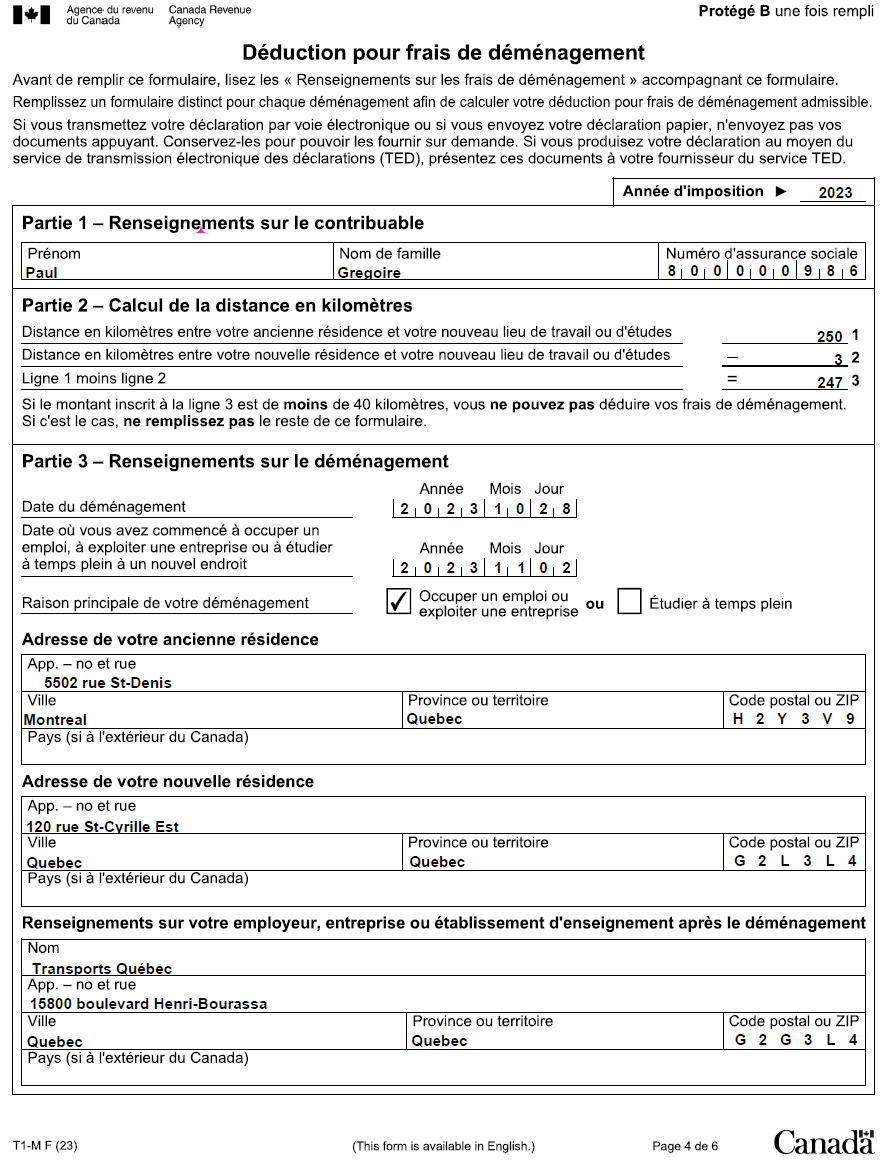
\includegraphics[height=\textheight]{exercice/3-5/Q5/T1-M-p4.png}

\noindent
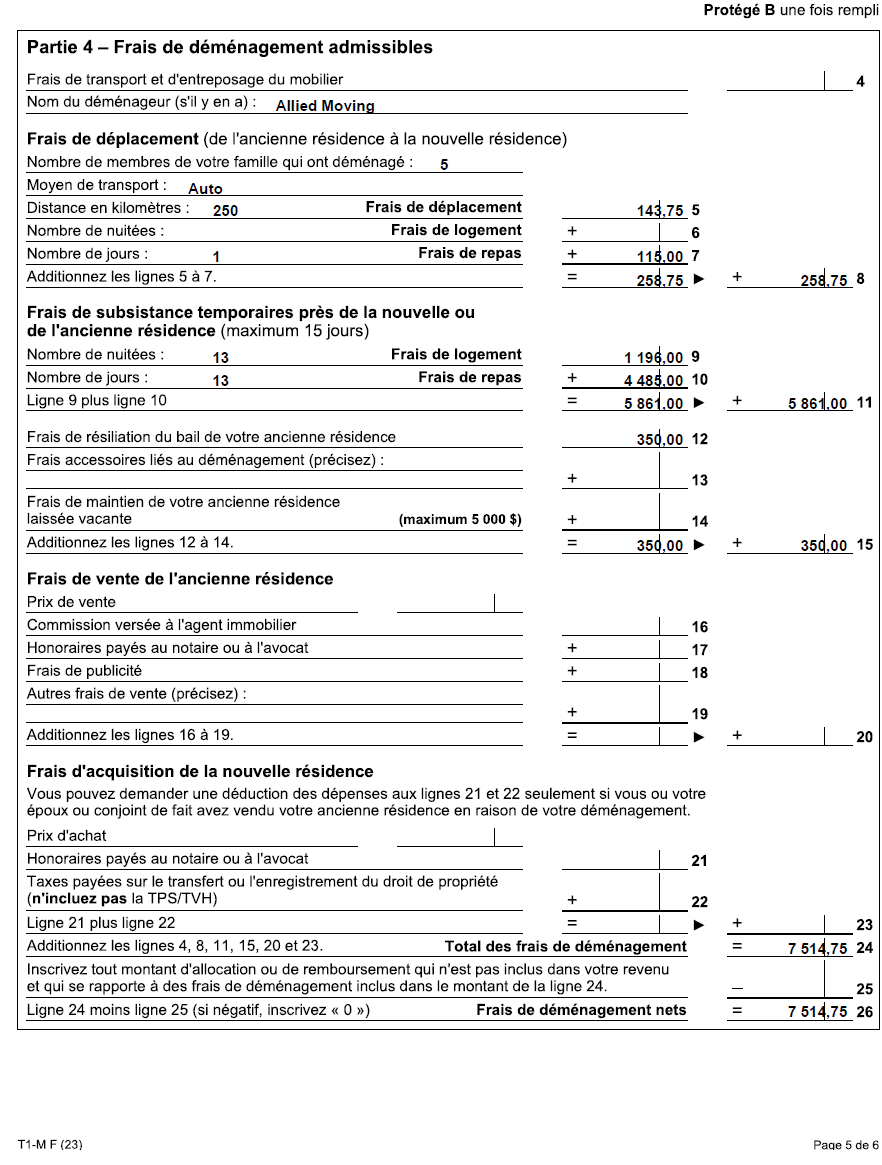
\includegraphics[height=\textheight]{exercice/3-5/Q5/T1-M-p5.png}

\noindent
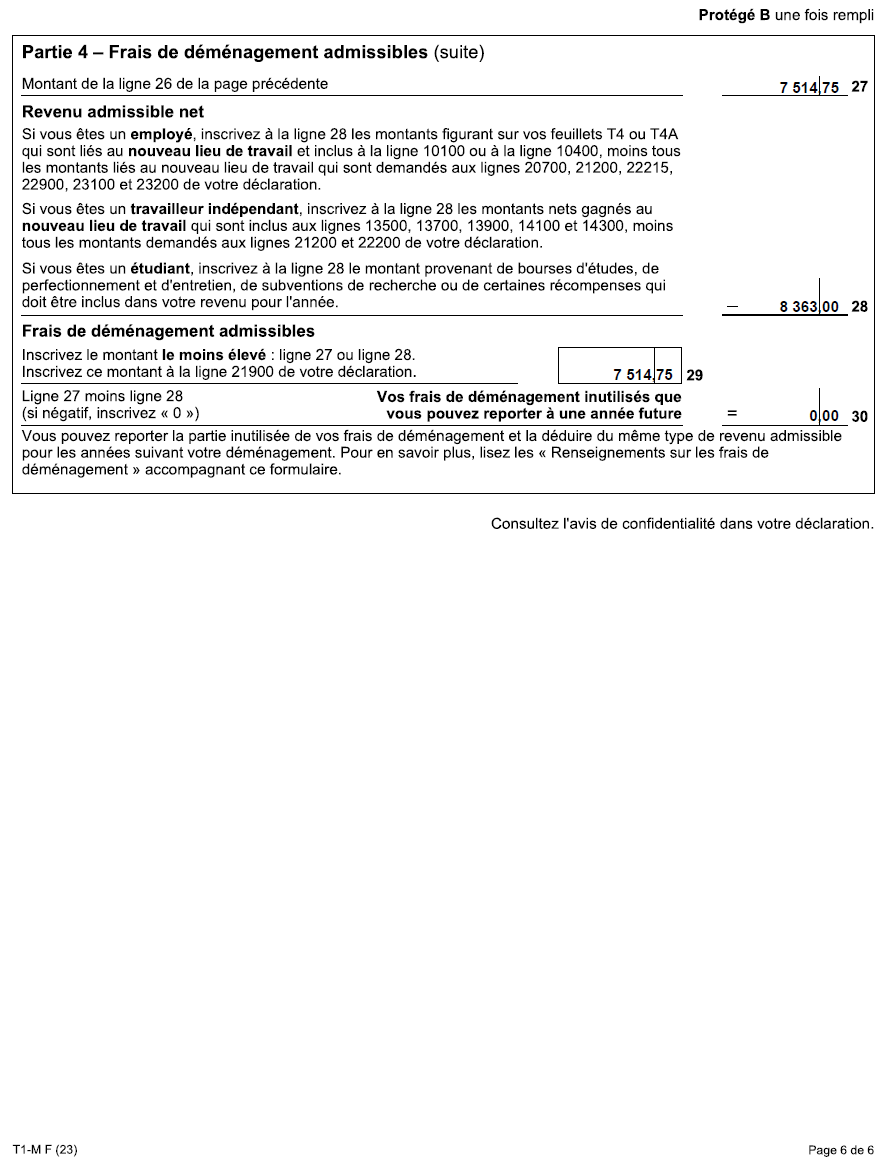
\includegraphics[height=\textheight]{exercice/3-5/Q5/T1-M-p6.png}

\noindent
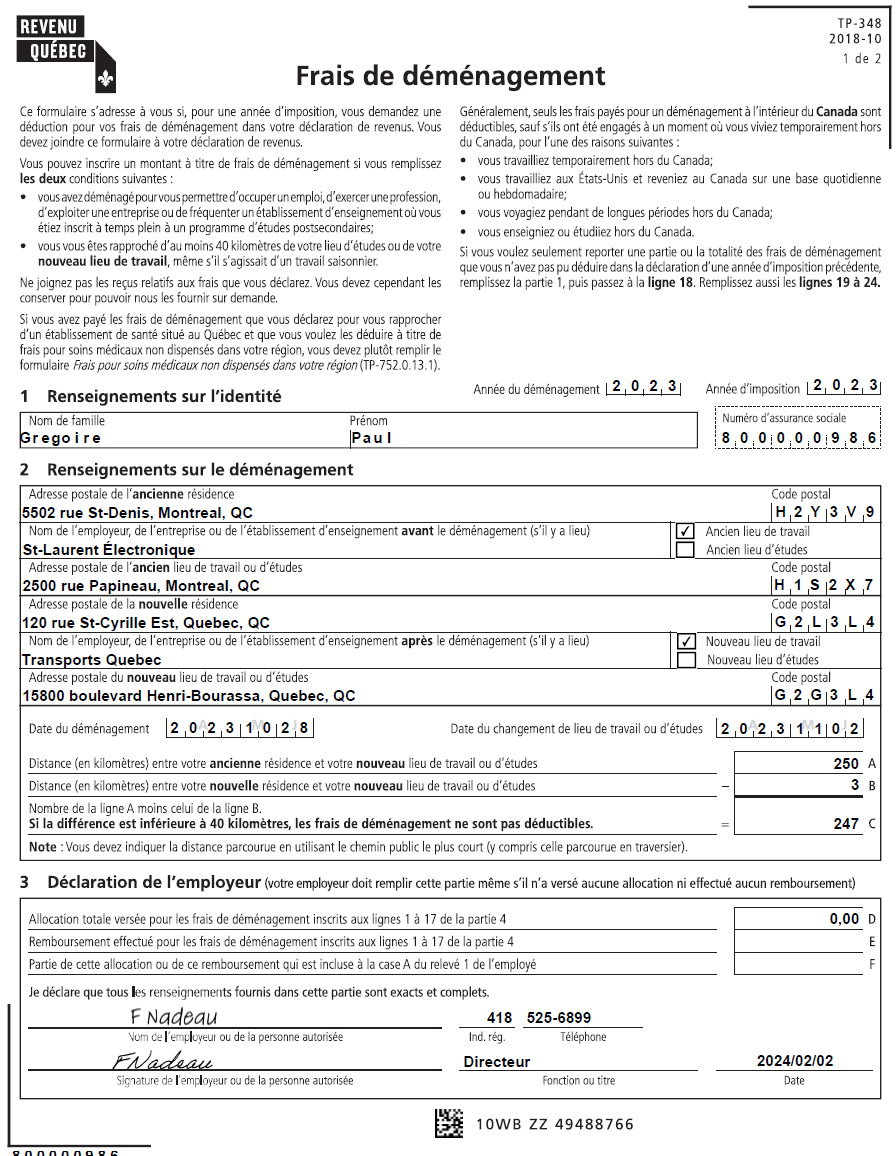
\includegraphics[height=\textheight]{exercice/3-5/Q5/TP-348-p1.png}

\noindent
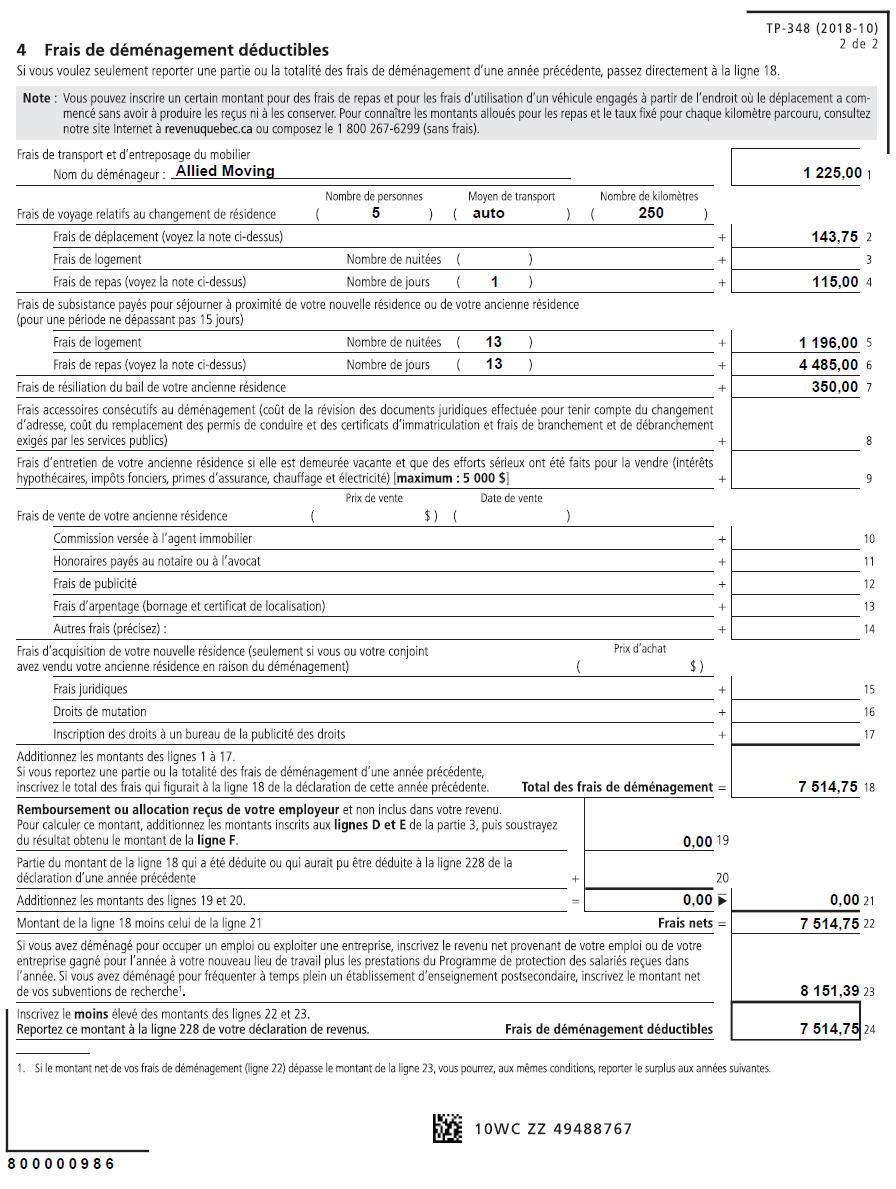
\includegraphics[height=\textheight]{exercice/3-5/Q5/TP-348-p2.png}



\section{Sommaire du chapitre 3}
\begin{itemize}
	\item La distinction entre une déduction et un crédit d'impôt.
	\item La \og Déduction pour travailleur \fg{} au Québec seulement.
	\item Les régimes de retraite des gouvernements - RPA et RVÉR.
	\item La complexité du calcul des cotisations syndicales et professionnelles.
	\item L'admissibilité des frais de déménagement.
	\item Le remboursement de salaire et de prestation.
	\item L'impact des déductions spécifiques sur le revenu net.
	\item Un petit aperçu des déductions spécifiques.
	\item L'impact des déductions spécifiques sur le revenu imposable.
	\item Montant de l'impôt à payer.
	\item L'utilisation des crédits d'impôt principalement au fédéral.
	\item Les cotisations aux programmes sociaux (RRQ, AE et RQAP).
	\item Le \og Montant canadien pou emploi \fg{} au fédéral seulement.
	\item Les crédits d'impôt prévus pour les volontaires des services d'urgence.
	\item Les crédits d'impôt pour les nouveaux diplômés travaillant dans les régions ressources éloignées du Québec.
\end{itemize}



\section{Problème de révision du chapitre 3}
\subsection{Renseignements personnels du couple}
\begin{center}
	\begin{tabular}{|l|c|c|}
		\hline
		\rowcolor{LightGreen} \textbf{Description} & \textbf{Contribuable 1} & \textbf{Contribuable 2}  \\ \hline
		Nom                                        &    Donna St-Laurent     &     Ginette Bernard      \\ \hline
		NAS                                        &       801 115 296       &       801 115 304        \\ \hline
		Date de naissance                          &      10 avril 1991      &       24 mars 1991       \\ \hline
		Statut civil                               &       \multicolumn{2}{c|}{Conjoints de fait}       \\ \hline
		Sexe                                       &            F            &            F             \\ \hline
		Province de résidence                      &           QC            &            QC            \\ \hline
		Langue                                     &            F            &            F             \\ \hline
		Téléphone                                  &        \multicolumn{2}{c|}{(514) 737-2899}         \\ \hline
		Adresse courriel                           & \multicolumn{2}{c|}{donna.st-laurent@videotron.ca} \\ \hline
		Consentement à l'envoi de communications   &           Oui           &           Oui            \\
		par voie électronique uniquement           &                         &                          \\ \hline
		Régime d'assurance médicaments             &          RAMQ           &           RAMQ           \\ \hline
		Adresse                                    &    \multicolumn{2}{c|}{1896 avenue Des Chênes,}    \\
		                                           &           \multicolumn{2}{c|}{appt 505,}           \\
		                                           &     \multicolumn{2}{c|}{Montréal, QC, H2L 4J8}     \\ \hline
		Citoyenneté canadienne                     &           Oui           &           Oui            \\ \hline
		Élections Canada                           &           Oui           &           Oui            \\ \hline
		Biens étrangers                            &           Non           &           Non            \\ \hline
		Revenu                                     &           Oui           &           Non            \\ \hline
	\end{tabular}
\end{center}


\subsection{Feuillets}
\noindent
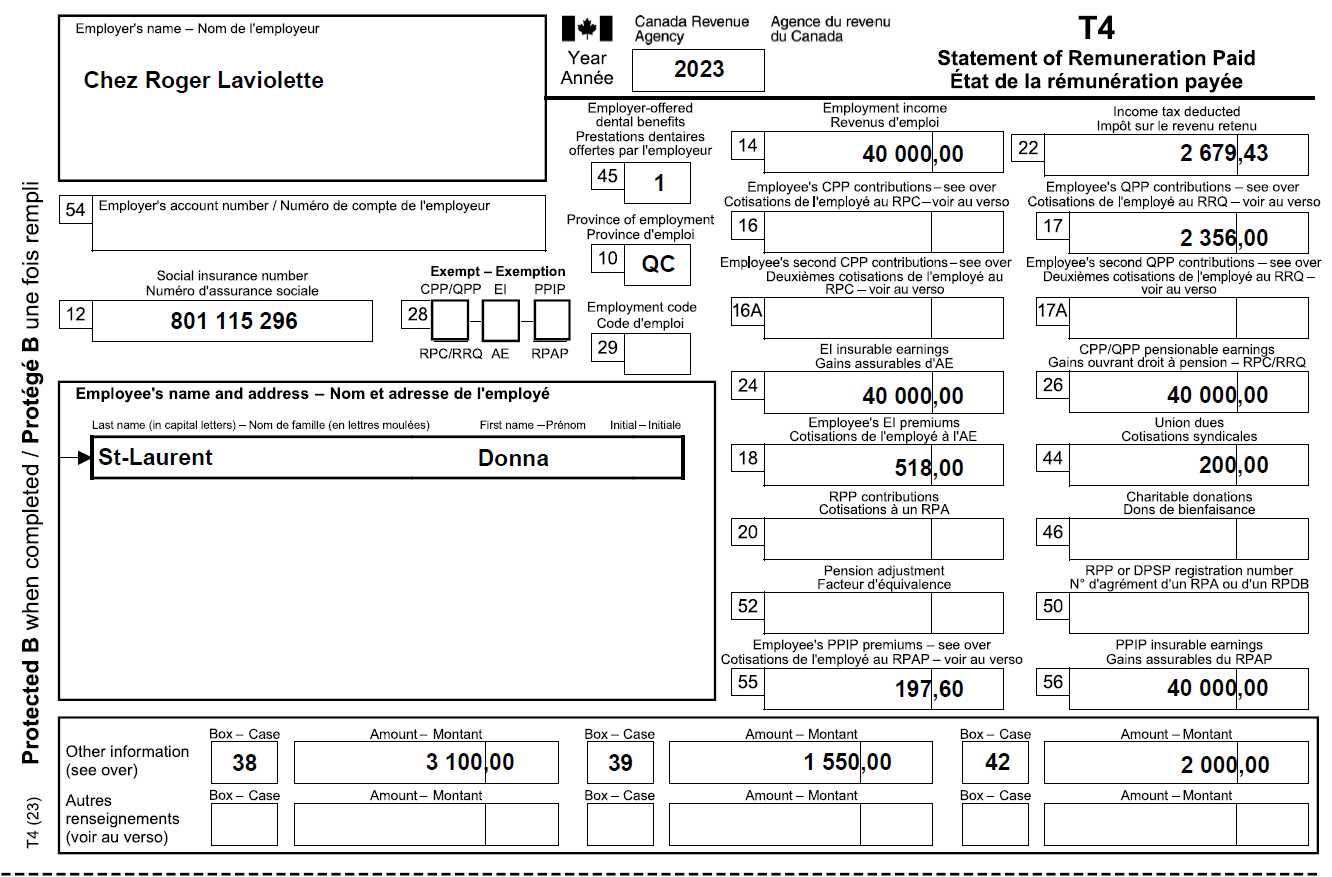
\includegraphics[width=\textwidth]{probleme/chapitre-3/T4.png}

\noindent
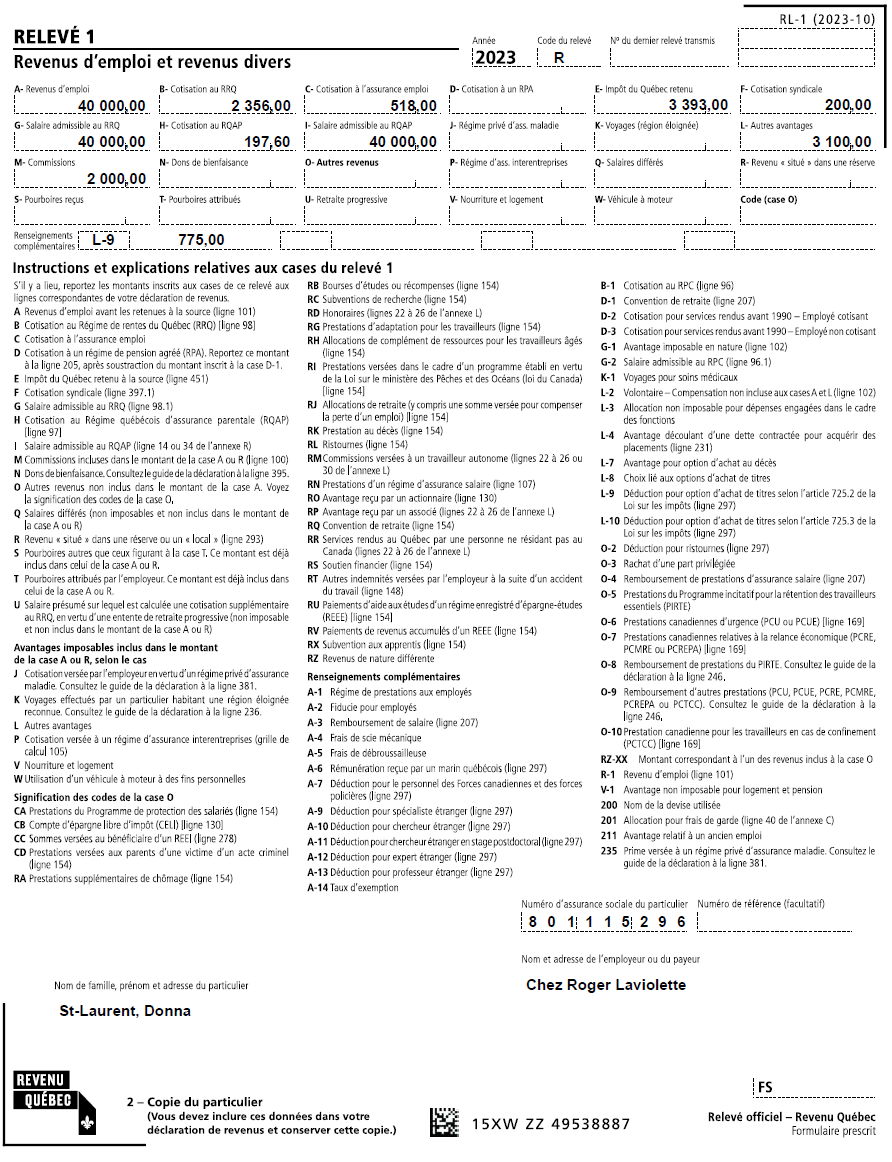
\includegraphics[width=\textwidth]{probleme/chapitre-3/RL1.png}


\subsection{Questions}
Complétez les étapes~2 à 4 de la \href{https://www.canada.ca/fr/agence-revenu/services/formulaires-publications/trousses-impot-toutes-annees-imposition/trousse-generale-impot-prestations/quebec/5005-r.html}{5005-R F} et pages~2 et 3 jusqu'à la ligne~299 de la \href{https://www.revenuquebec.ca/documents/fr/formulaires/tp/2023-12/TP-1.D%282023-12%29.pdf}{TP-1}.

\setcounter{question}{0}
\begin{question}
	À l'aide des renseignements figurant sur les feuillets d'impôt, calculez le trop-perçu au titre du RRQ, s'il y a lieu.
\end{question}
TP1, ligne 452 = Annexe 8, ligne 14 = 20,00

Gains ouvrant droit à pension RRQ (T4 case 26) = \numprint{40000,00}

Cotisations de l’employé au RRQ (T4 case 17) = \numprint{2356,00}

Cotisations requises = (\numprint{40000,00} - \numprint{3500,00}) $\times$ 6,4 \% = \numprint{2336,00}

\begin{question}
	Effectuez les entrées appropriées aux lignes suivantes de la T1 et TP-1 de Donna.
	\begin{itemize}
		\item TP-1: lignes 98, 98.1 et 452 
		\item T1: lignes 30800 et 22215
	\end{itemize}
\end{question}
\begin{itemize}
	\item TP-1
	\begin{description}
		\item[Ligne 98] \numprint{2356,00} (Cotisation au RRQ, relevé 1, case B )
		\item[Ligne 98.1] \numprint{40000,00} (Salaire admissible au RRQ, relevé 1, case G)
		\item[Ligne 452] 20,00 (Cotisation payée en trop au RRQ)
	\end{description}
	\item T1
	\begin{description}
		\item[Ligne 30800] \numprint{1971,00} (Cotisations de base RRQ, Annexe 8, (\numprint{40000,00} -  \numprint{3500,00}) $\times$ 5,4~\%)
		\item[Ligne 22215] 365,00 (Déduction pour les cotisations bonifiées au RRQ, Annexe 8, (\numprint{40000,00} -  \numprint{3500,00}) $\times$ 1 \%)
	\end{description}
\end{itemize}

\begin{question}
	Calculez le paiement en trop à l'AE, le cas échéant, à l'aide de l'annexe 10.
\end{question}
Ligne 18 = \numprint{40000,00} (T4 case 24)

Ligne 20 = 508,00 = Ligne 22

Ligne 21 =  518,00 (T4 case 18)

Ligne 23 = 518,00 - 508,00 = 10,00

\begin{question}
	Quelles inscriptions devez-vous faire sur les déclarations fédérale et provinciale de Donna à l'égard de ses cotisations à l'AE?
\end{question}
31200 - Crédit d'impôt non remboursable : 40 000 (case 24) * 1,27 \% = 508,00

45000 - Paiement en trop d'AE : 10,00

Rien au provincial

\begin{question}
	Calculez le paiement en trop au RQAP, le cas échéant.
\end{question}
Hors Québec, les prestations d'assurance parentale sont assumées par l'AE.

Au Québec, elles sont assumées par le RQAP.

Cotisation RQAP dû = \numprint{40000,00} (case I du RL-1) $\times$ 0,494 \% = 197,60

Cotisation RQAP payée = case H = 197,60 ; pas de paiement en trop

\begin{question}
	Effectuez les entrées appropriées aux lignes suivantes de la T1 et TP-1 de Donna.
	\begin{itemize}
		\item TP-1: lignes 97 et 457
		\item T1: ligne 31205
	\end{itemize}
\end{question}
\begin{itemize}
	\item TP-1
	\begin{description}
		\item[Ligne 97] 197,60 (Cotisation au RQAP, relevé 1, case H)
		\item[Ligne 457] 0,00 (Cotisation payée en trop au RQAP)
	\end{description}
	\item T1
	\begin{description}
		\item[Ligne 31205] 3197,60 (Cotisations au RPAP, T4, case 55)
	\end{description}
\end{itemize}

\begin{question}
	Ginette n'a eu aucun revenu durant l'année. Est-ce qu'elle doit produire une déclaration de revenus? Expliquez votre réponse.
\end{question}
Oui, T1, crédit pour la TPS (T1), crédit d'impôt pour solidarité + transfert crédits d'impôt non remboursable (TP-1)
